%%% Dateikodierung: UTF-8

%%% Magic Comments zum Setzen der korrekten Parameter in kompatiblen IDEs
% !TeX encoding = utf8
% !TeX program = pdflatex 
% !TeX spellcheck = de_DE
% !BIB program = biber

\documentclass[bachelor,german,smartquotes]{hgbthesis}
% Zulässige Optionen in [..]: 
%    Typ der Arbeit: 'diploma', 'master' (default), 'bachelor', 'internship'
%		 Zusätzlich für ein Thesis-Exposé: 'proposal' (für 'bachelor' und 'master')
%    Hauptsprache: 'german' (default), 'english'
%    Option zur Umwandlung in typografische Anführungszeichen: 'smartquotes'
%    APA Zitierstil: 'apa'
%%%-----------------------------------------------------------------------------

\RequirePackage[utf8]{inputenc} % bei Verw. von lualatex oder xelatex entfernen!

\graphicspath{{images/}}  % Verzeichnis mit Bildern und Grafiken
\logofile{logo}           % Logo-Datei: images/logo.pdf (kein Logo: \logofile{})
\bibliography{references} % Biblatex-Literaturdatei (references.bib)

%%%-----------------------------------------------------------------------------
\begin{document}
%%%-----------------------------------------------------------------------------

%%%-----------------------------------------------------------------------------
% Angaben für die Titelei (Titelseite, Erklärung etc.)
%%%-----------------------------------------------------------------------------

\title{Vergleich der Extension-APIs in Visual Studio Code und IntelliJ IDEA}
\author{Philipp Seiringer}
\programname{Software Engineering}

\programtype{Fachhochschul-Bachelorstudiengang}

\placeofstudy{Hagenberg}
\dateofsubmission{2024}{02}{01} % {YYYY}{MM}{DD}

\advisor{Dr. Josef Pichler} % optional

%\strictlicense % restriktive Lizenz anstatt Creative Commons (nicht empfohlen!)

%%%-----------------------------------------------------------------------------
\frontmatter                                       % Titelei (röm. Seitenzahlen)
%%%-----------------------------------------------------------------------------

\maketitle
\tableofcontents

\chapter{Kurzfassung}

Das Arbeiten mit IDEs kann durch die Entwicklung von 
Plugins oder Extensions verbessert werden. Die Entscheidung,
für welche Programmierumgebung ein Plugin entwickelt werden soll,
ist, vor allem ohne Vorerfahrung, allerdings nicht trivial.

Es werden daher die Extension-APIs in den IDEs Visual Studio Code
und IntelliJ IDEA analysiert und verglichen. Für den Vergleich
wird ein Katalog an Bewertungskriterien aufgestellt, an denen die
beiden Systeme gemessen werden können.

Um für den Vergleich eine praktische Grundlage zu schaffen, wird
ein prototypisches Plugin für beide Plattformen entwickelt. Aufgrund
der dabei gemachten Erfahrungen können die Bewertungskritierien
ausgeführt und verglichen werden. Durch das erarbeitete Wissen
kann effektiv eine Entscheidungsbasis für neue Plugin EntwicklerInnen
geschaffen werden.		
\chapter{Abstract}


\begin{english} %switch to English language rules
This should be a 1-page (maximum) summary of your work in English.
%und hier geht dann das Abstract weiter...
\end{english}

			

%%%-----------------------------------------------------------------------------
\mainmatter                             % Hauptteil (ab hier arab. Seitenzahlen)
%%%-----------------------------------------------------------------------------

\chapter{Einleitung}
\label{cha:Einleitung}


\section{Motivation}
\label{sec:Motivation}

SoftwareentwicklerInnen arbeiten täglich mit verschiedensten 
Werkzeugen und Entwicklungsumgebungen, sogenannten IDEs 
(=Integrated Development Environment). Diese Plattformen 
bieten teils sehr unterschiedliche Funktionalitäten, die 
die Softwareentwicklung erleichtern sollen. Dabei bieten 
sie Unterstützung für verschiedenste Programmiersprachen 
und Technologien und binden zahlreiche Werkzeuge für 
spezifische Anwendungsfälle ein. Aufgrund des immer rascher
werdenden Entstehens von neuen Technologien bieten mehr 
und mehr IDEs Möglichkeiten zur Entwicklung von eigenen 
Plugins, welche dann auch an andere EntwicklerInnen 
bereitgestellt werden können. So können in kürzester 
Zeit neue Technologien unterstützt werden und 
EntwicklerInnen haben selbst die Macht darüber zu 
entscheiden, welche Plugins sie nutzen möchten und 
welche nicht.

Vor der Entwicklung solcher Plugins ist es wichtig 
zu entscheiden für welche IDE das Plugin erstellt 
werden soll. Dabei spielen Aspekte wie zum Beispiel 
die Einfachheit und Flexibilität in der Entwicklung, 
der Umfang an angebotener Funktionalität, die Möglichkeit % //TODO rewrite?
die Nutzerinteraktion und somit die User Experience 
zu steuern und viele weitere eine Rolle. 
Diese Bachelorarbeit versucht in diesen Bereichen 
einen Überblick zu schaffen und vergleicht hierfür 
die Plugin Entwicklung in zwei der momentan beliebtesten 
IDEs, Visual Studio Code und IntelliJ IDEA. Durch den 
Vergleich der beiden Produkte und dem Herausarbeiten 
und Aufbereiten der Unterschiede wird es anderen 
EntwicklerInnen erleichtert diese Entscheidung zu treffen.


\section{Ziel}
\label{sec:Ziel}

\section{Aufbau}
\label{sec:Aufbau}
\chapter{Grundlagen der Plugin-Entwicklung}
\label{cha:Grundlagen}

\section{Entwicklungsumgebungen}
\label{sec:Entwicklungsumgebungen}

\subsection{Visual Studio Code}

Die erste offizielle Version von Visual Studio Code, häufig 
abgekürzt auch als VS Code, wurde im April 2016 \cite{VSCodeReleaseDate}
von Microsoft veröffentlicht. Die Idee hinter VS Code
war, einen möglichst einfachen Code Editor anzubieten, 
welcher nur die wichtigsten und besten Funktionen für EntwicklerInnen 
beinhaltet. Es hob sich somit von anderen Entwicklungsumgebungen (engl. IDEs)
wie der Visual-Studio-Reihe von Microsoft ab, da es ein sehr 
leichtgewichtiger Editor war, welcher trotzdem mit einer großen 
Menge an Programmiersprachen arbeiten konnte und für diese auch 
Microsofts automatische Codevervollständigung namens „IntelliSense“ 
unterstützte. Weiters war Visual Studio Code das erste Produkt der Visual 
Studio Familie, welches plattformübergreifen für Windows, Linux und macOS 
angeboten wurde \cite{VSCodePreview}.

Aus den Stack Overflow Developer Surveys\cite{StackOverflowSurvey,StackOverflowSurvey2023}
der vergangenen Jahre kann 
der rasche Aufstieg von VS Code beobachtet werden. Während es im 
Jahr der Veröffentlichung nur von etwa 7,2 Prozent der EntwicklerInnen 
genutzt wurde, war es zwei Jahre später bereits (wenn auch knapp) 
die meistgenutzte IDE mit 34,9 \%. In der aktuellsten Umfrage von 
2023 war es der klare Sieger und wurde vom 73,71\% der Abstimmenden 
aktiv genutzt\cite{StackOverflowSurvey,StackOverflowSurvey2023}.

Ein Grund für diesen Erfolg mag vermutlich die Möglichkeit 
zur Entwicklung und zum Anbieten von Extensions sein. Durch die direkte 
Einbindung des Visual Studio Marketplace in VS Code bildete sich über die 
Jahre eine große Community, die eine enorme Anzahl von Extensions 
entwickelt, verbessert und betreut. Durch solche, oft 
von der Community erstellte, Extensions kann VS Code auch eine 
enorme Anzahl von Programmiersprachen unterstützen.


\subsection{IntelliJ IDEA}

IntelliJ IDEA wurde erstmals im Januar 2001 \cite{IntelliJIDEAWikipedia,IntelliJReleasePage}
von dem Unternehmen 
JetBrains veröffentlicht. Im Gegensatz zu VS Code handelt 
es sich bei IntelliJ um eine vollausgetattetes Integrate Development Environment (IDE),
welche speziell auf die Entwicklung 
von Programmen in den Programmiersprachen Java, Kotlin und Groovy ausgelegt ist. 
IntelliJ IDEA wird in einer freien, Open Source 
\enquote{Community Edition} sowie in einer kommerziellen Form 
\enquote{IntelliJ IDEA Ultimate} angeboten \cite{HagosTed2022BII:}. 

Aufgrund der Spezialisierung auf JVM-kompatible Sprachen unterstützt 
die IntelliJ Community Edition nur eine relativ kleine Auswahl an 
Sprachen, Frameworks und Build Tools. Während IntelliJ IDEA Ultimate 
den Umfang an Features schon deutlich erweitert, bietet JetBrains auch 
noch weitere kommerzielle IDEs an. Diese sind alle für unterschiedliche 
Programmiersprachen oder Sprachfamilien ausgelegt. Einige der bekanntesten 
sind dabei CLion für die Sprachen C und C++, Rider für die .NET Sprachen, 
PhpStorm für PHP und WebStorm für JavaScript. Zum aktuellen 
Zeitpunkt sind es insgesamt elf verschiedene IDEs, die von JetBrains 
angeboten werden und die alle auf der IntelliJ Platform basieren. Das 
bedeutet nicht nur, dass sich all diese IDEs in der Verwendung und im 
Aussehen sehr ähnlich sind, sondern auch, dass ein Plugin, welches für 
die allgemeine IntelliJ Platform entworfen wurde, 
auch für mehrere IDEs dieser Plattform veröffentlicht werden kann \cite{IntelliJSDKDocumentation}.

Im Gegensatz zu Visual Studio Code ist IntelliJ ein schwergewichtiger
Editor, der sehr viel Funktionalität schon von Grund auf eingebaut 
hat. Die EntwicklerInnen sind hier nicht so stark auf Plugins angewiesen.
Dies lässt sich auch durch die Anzahl von Plugins erkennen, die auf dem 
JetBrains Marketplace angeboten werden. Für die IntelliJ Platform gibt 
es aktuell etwas über 7.500 Plugins, die in die IDE integriert werden können 
\cite{IntelliJMarketplace}.
Für Visual Studio Code sind es hingegen inzwischen über 51.000 Extensions
\cite{VSCodeMarketplace}.


\section{Programmiersprachen}
\label{sec:Programmiersprachen}

\subsection{TypeScript}

Die Programmiersprache TypeScript wurde erstmalig am 1. Oktober 2012 
\cite{TypeScriptCodePlexArchived} von 
Microsoft in Form eines Open-Source-Projekts veröffentlicht. Entworfen wurde sie 
von Anders Hejlsberg, der zuvor auch die Programmiersprache C\# entworfen hatte. 

Die grundsätzliche Idee der Sprache ist, eine typsichere, kompilierte, und somit 
bessere Version von JavaScript zu sein. JavaScript ist aufgrund des Erfolgszugs
des World Wide Web zu einer sehr wichtigen Sprache geworden und war auch schon 2012 
aus den TOP-Listen für Programmiersprachen nicht mehr wegzudenken 
\cite{StackOverflowSurvey,TIOBEIndex,PYPL}. 
Webseiten setzen heute sehr stark auf JavaScript, um durch interaktive Elemente 
die User Experience zu verbessern oder um neue Funktionalität anbieten zu können. 
Durch Node.js kann JavaScript nicht nur im Browser 
verwendet werden, sondern es können auch Desktop-, Server- oder mobile-Anwendungen 
in JavaScript entwickelt werden \cite{rozentals2017mastering}.
Durch diesen großen Umfang an Möglichkeiten, die 
JavaScript dadurch bietet, werden auch immer größere Projekte damit entwickelt. 
Und hier kommen die großen Schwächen von JavaScript zu tragen. 
Je größer die Projekte werden und je mehr EntwicklerInnen an einem Projekt 
mitarbeiten, desto mehr Fehler entstehen aufgrund der fehlenden Typsicherheit
und der fehlenden statischen Überprüfungen (wie zum Beispiel bei einem Compiler). 
Beide Schwachstellen versucht TypeScript auszubessern.

TypeScript Quellcode wird mithilfe des TypeScript Compilers \emph{tsc} in JavaScript 
Dateien transpiliert. Dadurch kann auf die Popularität und Verbreitung von JavaScript 
aufgebaut werden. TypeScript ist überall dort verwendbar, wo JavaScript 
ausführbar ist. Weiters ist TypeScript eine echte Übermenge von JavaScript. 
Es gilt also: „Any valid .js file can be renamed .ts and be compiled with other 
TypeScript file.” \cite{MaharryDanTR}. 

Jedoch bietet TypeScript eine Menge von Vorteilen 
gegenüber Javascript.
\begin{itemize}
  \item Durch den Kompilierschritt mit dem tsc Compiler wird der 
    Code vor der Ausführung automatisch auf Validität geprüft. 
    Es entfällt also die Notwendigkeit für einen zusätzliches Werkzeug 
    zur statischen Programmanalyse, wie JSLint. 
    Dieser Kompilierschritt kann natürlich auch in eine 
    CI/CD Pipeline eingebunden werden, um auch bei Änderungen in einem
    Repository Informationen über die Gültigkeit des Quellcodes zu erhalten.
  \item Durch die statische Typisierung können Programmierfehler bezüglich
    der Verwendung von Variablen vermieden werden. Auch die Unterstützung 
    durch verschiedene IDEs, zum Beispiel mittels IntelliSense kann durch 
    Typen verbessert werden. Dies ist nicht nur bei der Zusammenarbeit hilfreich, 
    sondern kann auch die Arbeit jeder einzelnen EntwicklerIn beschleunigen.
  \item In TypeScript können Klassen erstellt werden, deren Eigenschaften mit 
    Zugriffsmodifikatoren (\emph{private}/\emph{public}) versehen sind.
  \item TypeScript unterstützt Vererbung, Schnittstellen und generische Programmierung.
  \item In TypeScript können bereits bestehende JavaScript-Bibliotheken 
    verwendet werden. Weiters ist es möglich, durch zusätzliche Dateien 
    Typinformationen zu \linebreak
    JavaScript-Bibliotheken zu liefern.
\end{itemize}

\subsection{Java}

Die Entwicklung der Programmiersprache Java begann im Jahr 1991. Java 
wurde von James Gosling, Mike Sheridan und Patrick Naughton entworfen \cite{WinnieDoug2021EJfA}.
Java wurde erstmals im Jahr 1995 von Sun Microsystems veröffentlicht. 
Im Januar 2010 wurde Sun Microsystems von der Oracle Corporation übernommen, 
welche seitdem auch Java weiterentwickelt.

Das Design und vor allem die Syntax der Sprache war stark von C und C++ inspiriert \cite{ArnoldKen1996TJpl}, 
um EntwicklerInnen einen leichten Umstieg auf die neue Sprache Java zu ermöglichen. 
Allerdings versuchte Java die teils sehr komplexen (wenn auch effektiven) 
Sprachfeatures von C++ etwas zu vereinfachen. Java sollte eine einfach, objektorientierte 
und robuste Sprache werden. Die Funktionalität die Java zu dem großen Erfolg verhalf, 
den sie später hatte, war das Prinzip
\begin{quote}\begin{english}\enquote{write once, run anywhere}\end{english}\end{quote}
(WORA) \cite{SharanKishori2022BJ1f}. 

Im Gegensatz 
zu den zuvor gängigen Programmiersprachen muss Java nämlich nicht für bestimmte 
Hardwarearchitekturen kompiliert werden. Java-Programme werden in eine 
Zwischensprache, den sogenannten Java Bytecode, kompiliert. Dieser Bytecode
kann dann von einer Java Virtual Machine (JVM) ausgeführt werden. Diese JVM ist
im Grunde ein eigenständiges Programm, welches mit der Java Runtime Environment 
(JRE) mitgeliefert wird. Ein kompiliertes Java-Programm kann also auf 
allen Geräten ausgeführt werden, auf denen eine passende JRE installiert ist. 
So ist es zum Beispiel auch möglich, Java für die Entwicklung von Android nativen
Apps auf Mobilgeräten zu benutzen.

Ein weiterer Vorteil gegenüber älteren Sprachen wie C++ ist die
automatisierte Speicherverwaltung. Diese funktioniert mithilfe eines 
sogenannten \enquote{Garbage Collectors} welcher nicht mehr benötigten Speicher
am Heap bereinigt und freigibt. Man kann also beliebig neue Objekte im Speicher
allokieren und muss sich nicht um die Deallokierung der zuvor erstellten Objekte
kümmern. Auf diese Weise können häufige Programmierfehler wie Memory Leaks unterbunden werden.

Java unterstützt sowohl das objektorientierte, das prozedurale als auch das funktionale 
Programmierparadigma. Der Fokus liegt allerdings stark auf der Objektorientierung. 
Dazu bietet Java Möglichkeiten zur Abstraktion durch Verwendung von Klassen, Information Hiding
mithilfe von Zugriffsmodifikatoren (\emph{public}/\emph{private}/\emph{protected}/\linebreak
\emph{package}), Vererbung, 
Schnittstellen, Polymorphismus, Überladen von Methoden, generischer Programmierung, 
Ausnahmebehandlung und vieles mehr.

% //TODO OPTIONAL section: LSP

\section{Aufbau der Plugin API}
\label{sec:AufbauDerPluginAPI}

Um die Bezeichnungen für IntelliJ Plugins und VS Code Extensions zu vereinheitlichen,
wird in den folgenden Abschnitten und Kapiteln \emph{Plugin} als Überbegriff
verwendet, der auch VS Code Extensions einschließt.

\subsection{Visual Studio Code}

Visual Studio Code bietet für Plugins zwei Arten der
Interaktion, welche zusammenspielen, um Plugins zu ermöglichen. 
Das Extension Manifest und die eigentliche API.
\subsubsection{Extension Manifest} 
  Das Extension Manifest befindet sich in der Datei \emph{package.json}.
  In dieser werden statische Einstellungen vorgenommen und
  Metainformationen über das Plugin bekannt gegeben. So kann hier unter
  anderem Name, Beschreibung, Herausgeber und Lizenzvereinbarungen
  eingestellt werden. Weiters definiert das Manifest eine sogenannte
  JavaScript- oder TypeScript-Datei \emph{main}  und dazu passende
  \emph{Activation Events} und \emph{Contribution Points}.
  \begin{description}
    \item[Activation Events] bestimmen den Zeitpunkt, an dem das Plugin zum ersten Mal
      aktiviert wird. Dabei wird die \emph{activate} Funktion der zuvor definierten
      \emph{main}-Datei ausgeführt. Der Aktivierungszeitpunkt sollte immer so spät wie
      möglich gewählt werden, um VS Code möglichst wenig zu verlangsamen und
      das Plugin erst bei Bedarf (on demand) zu Laden. Allerdings
      muss die Aktivierung erfolgen bevor die erste Funktionalität des
      Plugins erwartet wird. Typische Aktivierungsereignisse sind \emph{onCommand}
      , \emph{onDebug}, \emph{onView} oder \emph{onStartupFinished}.
      Wurde das Plugin einmal aktiv, bleibt es auch aktiv bis VS Code wieder geschlossen
      wird oder das Plugin entfernt oder deaktiviert wird. Hierfür gibt es optional
      noch eine \emph{deactivate}-Funktion in der \emph{main}-Datei, welche für etwaige
      Aufräumarbeiten genutzt werden kann.
    \item[Contribution Points] legen fest, welche Funktionalität das Plugin anbietet
      und somit auch, welche zusätzlichen UI-Elemente
      dem Nutzer in VS Code angezeigt werden sollen.
      Hier ist es beispielsweise möglich, Visual Studio Code mit neuen Befehlen (\enquote{Commands}),
      Menüs und Submenüs, Views für das Anzeigen von Plugin-definiertem Content,
      Keyboard Shortcuts, Unterstützung für neue Sprache und vieles mehr auszustatten.
  \end{description}
\subsubsection{Visual Studio Code API} 
  Die eigentliche VS Code API kann in jeder TypeScript-Datei 
  (zum Beispiel auch in der Datei \emph{main}) genutzt werden. 
  Hierfür wird das Modul \emph{vscode} importiert. 
  Dieses beinhaltet eine vollständige Definition der angebotenen
  Schnittstelle, auf welche zugegriffen werden kann.
\begin{JsCode}
    import * as vscode from 'vscode';

    export function activate(context: vscode.ExtensionContext) {
      vscode.window.showInformationMessage('Hello World!');
    } 
\end{JsCode}
  Über diese API kann zum Beispiel festgelegt werden, durch welchen Code
  die zuvor definierten Contribution Points implementiert werden sollen.
  Der Plugin Code wird in VS Code nicht im selben Prozess wie das
  Hauptprogramm ausgeführt, sondern abgekapselt in einem seperaten 
  \enquote{extension host process}. Dadurch kann verhindert werden, dass
  Plugins die Performance und die Interaktivität von VS Code negativ beinflussen 
  \cite{VSCodeArchitecture,VSCodeApproachToExtensibility}.
\subsubsection{Ablauf}
  Wie in Abbildung \ref{fig:diagram_VSCodeExtensionArchitecture} zu sehen ist,
  analysiert VS Code zuerst das Extension Manifest des Plugins.
  Je nachdem welche Activation Points definiert sind, wird zu einem
  bestimmten Zeipunkt die \emph{activate}-Funktion aufgerufen. In dieser 
  können dann mithilfe der API Event Handler registriert werden. 
  Die registrierten Handler werden dann während der Ausführung und Verwendung
  von VS Code aufgerufen und können so beliebigen Code ausführen.
  \begin{figure}
    \centering
    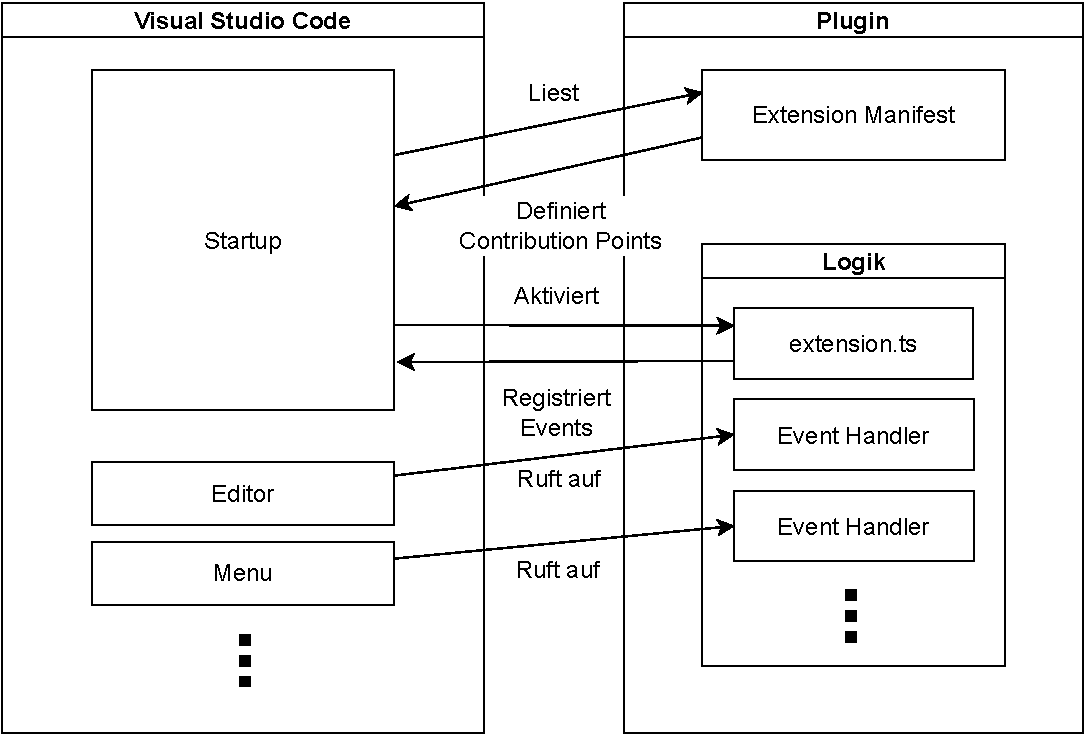
\includegraphics[width=.95\textwidth]{diagram_VSCodeExtensionArchitecture}
    \caption{Übersicht über den Ablauf eines VS Code Plugins.}
    \label{fig:diagram_VSCodeExtensionArchitecture}
  \end{figure}   

\subsection{IntelliJ IDEA}

Der Aufbau der Plugin-Architektur wirkt bei IntelliJ im ersten Moment 
gleich wie bei VS Code. Es gibt auch hier ein \emph{Plugin Configuration File}, 
sowie ein Modul mit API Schnittstellen.
Der große Unterschied liegt allerdings in der Funktionsweise und der Interaktion
mit den Plugins sowie der Art, wie der auszuführende Code angegeben wird.
\subsubsection{Plugin Configuration File}
  Die Konfiguration eines Plugins liegt in der Datei \emph{plugin.xml} und
  beinhaltet, äquivalent zum Extension Manifest in VS Code, alle für das Plugin
  notwendigen Meta-Informationen. So können auch hier Werte wie der Name,
  eine Beschreibung und die aktuelle Versionsnummer angegeben werden.
  Für die Funktionen, die das Plugin mitbringt, gibt es Actions, Extension Points
  und Listener. Hier ist anzumerken, dass es sich sowohl bei den Extension Points
  als auch den Listenern immer um eine Zuordnung eines Interfaces
  (meist definiert von IntelliJ) zu einer Implementierung (definiert durch das Plugin)
  handelt. Weiters ist es nicht nötig einen speziellen Aktivierungszeitpunkt
  festzulegen, da die Zuordnung der auszuführenden Klassen sowieso durch 
  die Konfigurationsdatei festgelegt wird. Eine Besonderheit an IntelliJ ist,
  dass Plugins auch eigene Extension Points definieren können, um weiteren Plugins
  das Erweitern des ursprünglichen Plugins zu ermöglichen.
\subsubsection{IntelliJ Platform SDK}
  Die API für IntelliJ Plugins ist in mehreren Paketen des IntelliJ 
  Platform SDK enthalten. Diese API enthält auch die unterschiedlichen
  Interfaces, welche dann in Form von Extension Points oder Listenern implementiert
  werden können. Die Implementierung eines Plugins kann in den Sprachen Java
  und Kotlin erledigt werden. Da die Plugin API allerdings auf Java basiert, können
  nicht alle Sprachfeatures von Kotlin problemlos genutzt werden.
\subsubsection{Ablauf}
  Wie in Abbildung \ref{fig:diagram_IntelliJExtensionArchitecture} zu sehen ist,
  analysiert IntelliJ zuerst das Plugin Configuration File.
  Je nachdem, welche Funktionalität vom Plugin angeboten wird, werden
  von IntelliJ automatisch die entsprechenden Event Handler 
  auf die unterschiedlichen Extension Points registriert. 
  Die registrierten Handler werden dann während der Ausführung und Verwendung
  von IntelliJ aufgerufen und können so beliebigen Code ausführen.
  \begin{figure}
    \centering
    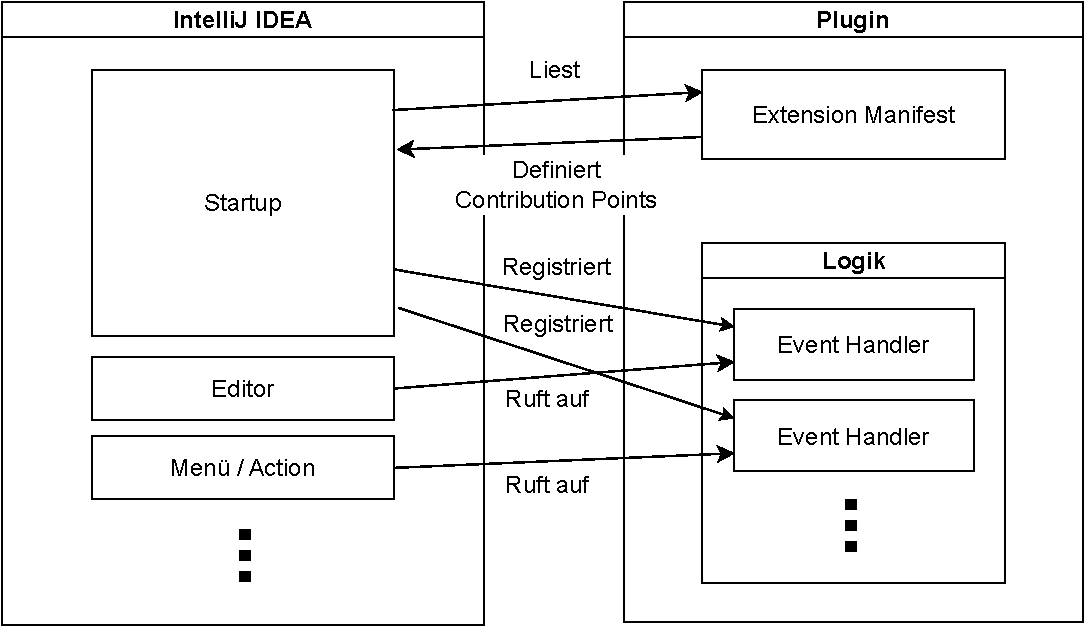
\includegraphics[width=.95\textwidth]{IntelliJExtensionArchitecture}
    \caption{Übersicht über den Ablauf eines IntelliJ Plugins.}
    \label{fig:diagram_IntelliJExtensionArchitecture}
  \end{figure}   

\section{Funktionalität der Plugin API}
\label{sec:FunktionalitätDerPluginAPI}

\subsection{Visual Studio Code}

Die VS Code API erlaubt es, VS Code durch Commands, Code Completion und Spracherweiterung, 
Themes, Custom Editor, Notebooks, Views, Source Control, Debugger, Tests und vielem mehr zu
erweitern. Um dies zu ermöglichen, werden unter anderem auch Einstellungen, Datenspeicherung
und verschiedene Arten der Ein- und Ausgabe von Daten bereitgestellt. In den folgenden Abschnitten
werden die wichtigsten Elemente genauer vorgestellt.

\subsubsection{Commands und Menüs}
  Commands ermöglichen es dem Plugin, bestimmten Code sozusagen \enquote{auf Befehl} auszuführen.
  So können häufig wiederkehrende Aufgaben der BenutzerInnen ganz einfach automatisiert werden.
  Um einen Command anzulegen, muss dieser im Extension Manifest definiert werden. Dabei muss
  das Plugin mindestens eine eindeutige Bezeichnung und zur Darstellung verwendeten Titel angeben.
  Optional können auch eine Kategorie, ein Icon und eine Kurzbezeichnung bestimmt werden. 
  Weiters ist es möglich eine Bedingung festzulegen, die beeinflusst, wann
  der Command verwendbar ist und wann nicht.
\begin{JsCode}
    "commands": [
      {
        "command": "vscodeplugindemo.helloWorld",
        "title": "Hello World",
      }
    ] 
\end{JsCode}

  Welcher Code dann ausgeführt wird, muss über die API festgelegt werden. So wird meist
  in der \emph{activate}-Funktion mithilfe von \emph{registerCommand} oder \emph{registerTextEditorCommand}
  ein Callback festgelegt, welches aufgerufen werden soll. Wichtig ist hier, dass
  die register-Funktionen ein Objekt retournieren, welches \emph{Disposable} implementiert.
  Dieses muss der API bekannt gegeben werden. 
  Die API kümmert sich dann auch um das Deaktivieren des Commands, falls zum Beispiel
  die Erweiterung deaktiviert werden sollte.
\begin{JsCode}
    context.subscriptions.push(vscode.commands.registerCommand('vscodeplugindemo.helloWorld', () => {
      vscode.window.showInformationMessage('Hello World from VsCodePluginDemo!');
    })); 
\end{JsCode}

  Um einen Command aufzurufen können die Nutzer direkt nach dem Command suchen (Tastenkombination Strg+Shift+P).
  Komfortabler ist es allerdings, den Nutzern direkt einen passenden Menüeintrag oder ein Keybinding
  bereitzustellen. Menüeinträge können dabei an verschiedenen Stellen in der
  Benutzeroberfläche eingehängt werden.
  Gängig sind hierfür die Titelleiste des Editors, verschiedene Kontext-Menüs, der Dialog
  zum Anlegen einer neuen Datei, die Titelleiste einer bestimmten View oder ein neues Submenü in der Menüleiste.
  Sowohl Menüs als auch Keybindings können im Manifest registriert werden.
  % // TODO OPTIONAL paragraph: about calling commands from code
\subsubsection{Spracherweiterungen}
  Ein wichtiger Teil der VS Code Plugin API sind Language Extensions. Visual Studio Code unterscheidet
  bei diesen Funktionen zwischen Highlighting, Language Features und Snippets.
  \begin{description}
    \item[Highlighting] 
      Das Syntax Highlighting wird in VS Code durch eine TextMate-\linebreak
      Grammatik erledigt \cite{TextMateGrammar}.
      Diese Grammatik wird dabei nicht nur für das Highlighting genutzt, sondern sie ist auch für das \enquote{Tokenization}
      zuständig. Durch eine Codeanalyse anhand der gegebenen Grammatik wird der Text in kleine 
      zusammengehörige Abschnitte (sogenannte Tokens) unterteilt. Diese Tokens werden zusätzlich noch 
      klassifiziert, sodass zum Beispiel zwischen Kommentaren, Zeichenkettenliteralen, regulären Ausdrücken und Code unterschieden werden kann.
      Die Grammatik wird hierfür in einer einfachen Json-Datei im Plugin Projektordner abgelegt und dann per Manifest
      unter dem Contribution Point \emph{grammar} eingebunden. Mithilfe solcher Grammatiken können auch bereits bestehende
      Grammatiken erweitert werden. Bei der Auswahl von Scopes, die durch die Grammatik definiert werden, sollte man sich
      an die Namenskonventionen von TextMate halten. Scopes mit diesem Namensschema werden auch von vielen Themes unterstützt werden.
      Um die Kategorisierung von bestimmten Tokens noch genauer zu erledigen, gibt es in VS Code auch \enquote{Semantic Highlighting}. 
      Es kann in der API ein \emph{DocumentSemanticTokensProvider} registriert werden,
      welcher den Code analysiert und zusätzliche (zum Beispiel kontextabhängige) Informationen über die Tokens bereitstellt.
    \item[Language Features] 
      Auch hier gibt es statisch definierte und programmatische Language Features.
      Statisch kann unter dem Contribution Point \emph{languages} eine Reihe von Informationen angegeben werden,
      die es VS Code erlauben, die User Experience stark zu verbessern. So kann man unter anderem festlegen,
      mit welchen Zeichen Kommentare eingeleitet werden, oder welche Klammern es gibt, damit VS Code das Zuklappen erlauben kann.
      Zusammengehörige Paare von Zeichen (also Klammern, Anführungszeichen, u.s.w.) können automatisch geschlossen werden.
      Und sogar für das automatische Einrücken der nächsten Zeile bei einem Zeilenumbruch kann eine Regel erstellt werden.
      Programmatisch ist das Erweitern von Language Features etwas komplexer, allerdings steigt auch die
      Menge an Möglichkeiten. In der API können verschiedene Provider registriert werden, durch die Features wie
      \enquote{Go to Definition}, \enquote{IntelliSense} Codevervollständigung oder diagnostische Fehleranalysen und
      entsprechende Verbesserungsvorschläge ermöglicht werden. Grundsätzlich ist es auch möglich, für einzelne
      Features einen Provider zu registrieren. Allerdings empfiehlt es sich, bei der Einbindung einer neuen
      Sprache, einen \enquote{Language Server} und das Language Server Protocol zu nutzen. Diese Lösung
      bringt nicht nur Performanceverbesserungen im Editor sondern der Language Server kann auch für 
      andere Editoren wiederverwendet werden, ohne dass er mehrfach implementiert werden muss. \cite{GunasingheNadeeshaan2022Lspa}.
      % //TODO OPTIONAL paragraph: results of existing lsp can probably be gotten by calling built-in commands. need some further research for this...
    \item[Snippets] 
      Snippets sind eine sehr einfache Form der Spracherweiterung. Es wird unter dem Contribution Point
      \emph{snippets} einfach eine Datei mit den Vorlagen angegeben. Eine Vorlage enthält dabei immer
      ein Kürzel für welches das Snippet vorgeschlagen werden soll, den zu ersetzenden Text und optional
      eine Beschreibung. Dabei können im Text auch Platzhalter genutzt werden an die der Cursor beim Einsetzen
      des Snippets springt.
  \end{description}
\subsubsection{Benutzereingaben}
  Für die Eingabe von Daten bietet VS Code die Quick Pick API, die File Picker API
  und den Configuration Contribution Point.
  \begin{description}
    \item[Quick Pick API] gibt dem Plugin eine Möglichkeit, den Nutzern ein einfaches Eingabefenster
      anzuzeigen. Dabei kann ein Fenster mit bereits vorgegebenen Auswahlmöglichkeiten durch
      den Aufruf von \emph{showQuickPick} oder \emph{createQuickPick} erstellt werden.
      Alternativ kann man mit den Funktionen \emph{showInputBox} oder \emph{createInputBox}
      die Nutzer auch selber einen Text eingeben lassen. Die show-Funktionen bieten dabei immer
      eine einfache vorgefertigte Implementierung an. Falls diese Option nicht ausreichend ist,
      kann mit den create-Funktionen auch eine komplexere Implementierung angegeben werden.
      Weiters kann auch eine Validierung des Inputs vorgenommen werden.
      Möchte man mehrere solcher Dialoge als Abfolge hintereinander anzeigen, so muss dies
      selber programmiert werden. Hierfür gibt es ein Beispiel namens \emph{quickinput-sample}
      im Repository \emph{vscode-extension-sample} \cite{VSCodeExtensionSamples}. 
    \item[File Picker API] erlaubt das Auswählen von Ordnern oder Dateien aus dem Dateisystem
      des Betriebssystems mit der Funktion \emph{showOpenDialog}. Dabei können Optionen angegeben
      werden, die zum Beispiel beeinflussen, ob Ordner und/oder Dateien gewählt werden dürfen, 
      ob mehrere Elemente selektiert werden dürfen oder ob nach Dateinamen gefiltert werden soll.
    \item[Configuration Contribution Point] ermöglichen das Festlegen von Einstellungen,
      die von den Nutzern eingegeben und vom Plugin ausgelesen werden können. Hier können
      Einstellungen vom Typ \emph{number}, \emph{string} und \emph{boolean} definiert werden, welche dann direkt
      im User Interface der VS Code Einstellungen bearbeitet werden können.
      Einfache \emph{object}- und \emph{array}-Eigenschaften können auch im UI dargestellt werden,
      allerdings dürfen diese keine verschachtelten Objekte oder Arrays enthalten.
      Ansonsten wird in den Einstellungen nur auf die manuell zu bearbeitende
      Datei \enquote{settings.json} verwiesen.
      Für die Validierung der Einstellungen können Validierungsproperties
      von JSON Schema verwendet werden. Es ist also zum Beispiel möglich,
      ein maximum/minimum, einen regulären Ausdruck oder ein enum Array
      mit erlaubten Werten anzugeben.
      Zusätzlich ist es zu jeder Einstellung möglich, einen Titel und eine Beschreibung
      anzugeben, wobei es sogar Beschreibungen gibt, welche Markdown-Formattierungen
      enthalten dürfen.
  \end{description}
\subsubsection{Ausgaben und Anzeigen}
  Um den BenutzerInnen auch Feedback über die Ausführung des Plugin-Codes zu geben, 
  ist in VS Code für drei allgemeine Anwendungsfälle vorgesorgt. 
  
  Um den BenutzerInnen eine kurze 
  Rückmeldung zu geben, können am besten Notifications genutzt werden. Diese zeigen eine kurze 
  Nachricht an, welche im Stil einer Information, einer Warnung oder einer Fehlermeldung 
  dargestellt werden kann. Um einen längeren Fluss von Ausgaben (wie zum Beispiel Log-Nachrichten 
  des Plugins) anzuzeigen, können Output Channels genutzt werden. An diese können Textzeilen nach 
  und nach angehängt werden und sie werden den BenutzerInnen dann in einer einfachen Textausgabe präsentiert. 
  In vielen Fällen reicht es schon als Feedback eine einfache Fortschrittsanzeige anzuzeigen. So kann den 
  BenutzerInnen klar gemacht werden, dass das Plugin immer noch arbeitet und noch kein Fehler aufgetreten 
  ist. Für diesen Anwendungsfall kann die Progress API genutzt werden.

  Eine etwas komplexere Anzeige bieten Views, die die sogenannte Workbench erweitern.
  Mit der Tree View API kann eine einfache Baumstruktur, ähnlich der 
  Dateiübersicht in der Explorer View, dargestellt werden. Für diese Implementierung
  muss ein \emph{TreeDataProvider} erstellt werden, welcher die Baumstruktur und
  den Inhalt vorgibt. Die Webview API bietet im Gegensatz dazu mehr
  Optionen. Diese kann in einer View eine Art \emph{iframe} anzeigen, in welchem
  dann HTML-Inhalte dargestellt werden können. Dabei kann auch JavaScript und CSS Code eingebunden
  werden, es können Nachrichten vom Plugin an die Webview und zurück geschickt werden, 
  es können Kontextmenüs in die View eingebunden werden und der Zustand der View
  kann persistiert werden.

\subsection{IntelliJ IDEA}

Das IntelliJ Platform SDK enthält einen sehr großen Umfang von Features und Extension Points,
die durch ein Plugin erweitert werden können. Einige wichtige Teile der API werden in den 
folgenden Abschnitten genauer beschrieben.

\subsubsection{Actions und Menüs}
  Actions in IntelliJ funktionieren fast ident zu den Commands aus VS Code. Es handelt sich um
  einen vom Plugin definierten Code-Block, welcher von den BenutzerInnen zum Beispiel über Menüeinträge
  angestoßen werden kann. Eine Action ist dabei eine einfache Java-Klasse, welche von der Klasse \emph{AnAction}
  abgeleitet wird. Dabei muss die Methode \emph{actionPerformed} überschrieben werden. Diese 
  enthält den Code, der von der Action ausgeführt wird. Optional sollte auch die
  \emph{update}-Methode überschrieben werden, durch welche bestimmt wird, wann die Action 
  aktiviert oder versteckt ist.

  Im Plugin Configuration File wird festgelegt, wo und wie die programmierten Actions angezeigt
  werden. Dabei wird im Abschnitt \emph{actions} ein \emph{action}-Element erstellt.
  Dieses hat für gewöhnlich eine eindeutige ID, eine Klasse mit der Code-Implementierung und
  einen Text, welcher zur Anzeige verwendet wird. Zusätzlich können eine Beschreibung und
  ein Icon festgelegt werden. Es können Gruppenzuordnungen bestimmt werden, die bestimmen,
  wo und wie die Action angezeigt wird. Es können Keyboard Shortcuts bestimmt werden. Und
  es kann mit \emph{override-text} ein alternativer Text angegeben werden, der nur an
  bestimmten Orten angezeigt wird.
  
\begin{XmlCode}
    <actions>
        <action id="my.simple.DemoAction"
                class="my.simple.DemoAction" 
                text="Demo Action">
            <add-to-group group-id="ToolsMenu" anchor="first"/>
        </action>
    </actions>
\end{XmlCode}

\subsubsection{Services}
  IntelliJ erlaubt es, Plugin Services zu definieren, welche dann auf drei Ebenen
  in jeweils zwei Varianten implementiert werden können. Instanzen solcher Services können
  dann an beliebigen Stellen im Plugin Code verwendet werden.

  Die Ebene auf der ein Service erstellt wird, bestimmt, wie viele Instanzen dieses 
  Services existieren können. Dabei gibt es das \emph{application-level}, welches den Service
  als globales Singleton anbietet. Und es gibt \emph{project-level} und \emph{module-level} Services, bei welchen
  für jedes geöffnetet Projekt bzw. Modul je eine Instanz des Services besteht. Allerdings 
  wird empfohlen, aus Effizienzgründen keine Services auf Modul-Level zu erstellen.
  
  In Bezug auf die Varianten gibt es Light Services und normale Services.
  Die Light Services sind einfache Klassen, welche mit der Annotation \emph{@Service}
  versehen sind. Light Services sind sehr effizient, allerdings gibt es einige Einschränkungen.
  So können beispielsweise keine anderen Services per Dependency Injektion injiziert werden.
  Vollwertige Services haben diese Einschränkungen nicht. Bei ihnen wird ein beliebiges Interface und
  eine dazugehörige Implementierung definiert. Diese werden daraufhin im Plugin Configuration File
  unter den Extension Points \emph{applicationService} oder \emph{projectService} registriert.
  Die Project-Level Services erhalten dabei sowohl als Light Service als auch als normaler Service, 
  eine Referenz auf das aktuelle Projekt.

\subsubsection{Listeners und Extension Points}

  Ganz ähnlich zu den vollwertigen Services funktioniert auch die Registrierung von Listenern
  und Extension Points. Allerdings gibt es hier bereits vorgefertigte Interfaces die implementiert
  werden müssen. Wurde die Implementierung dann in der Project Configuration registriert, wird
  sie zu den entsprechenden Zeitpunkten aufgerufen.
  
  Bei Extension Points gibt es die weitere Besonderheit, dass auch eigene Extension Points deklariert
  und im Plugin Code aufgerufen werden können. Diese werden dann für andere Plugins zur Erweiterung
  angeboten.

\subsubsection{PSI und Spracherweiterungen}

  PSI steht für Program Structure Interface und ist die Grundlage jeder Sprachunterstützung in
  IntelliJ. Immer wenn eine Datei mit Quellcode wird von IntelliJ geparsed wird, wird zugleich auch ein
  Objekt der Klasse \emph{PsiFile} generiert. 
  Dieses \emph{PsiFile}-Objekt enthält dann eine Baumstruktur von Objekten der Klasse
  \emph{PsiElement}, welche der Struktur des Quellcodes entspricht. 
  Die Blattknoten eines solchen Baumes entsprechen dabei
  für gewöhnlich einzelnen Tokens und Identifiern, die nicht mehr zerlegt werden können.
  Nach oben hin werden diese dann zu Anweisungen, Code-Blöcken, Methoden, Klassen u.s.w. gebündelt.
  Der Vorteil dieser \emph{PsiFile}-Objekte ist, dass sie von IntelliJ und auch von Plugins jederzeit
  verwendet werden können. Somit können unter anderem verschiedene Sprachfeatures sehr
  effizient implementiert werden.

  Um die IntelliJ Plattform mit einer neuen Sprache zu erweitern, muss zuerst die entsprechende
  Sprache und ihre Grammatik definiert werden. Die Grammatik hat dabei nicht nur die Aufgabe, die 
  Syntaxregeln einer neuen Sprache festzulegen. Durch sie wird auch die Struktur der Sprache festgestellt,
  was später für den Aufbau der PSI-Elemente wichtig ist. Hierfür wird eine Art der Backus Naur Form (BNF)
  verwendet, welche mit zusätzlichen Informationen gespickt wird \cite{mccracken2003backus,GrammarKit}. 
  So gibt es zum Beispiel Attribute
  wie private, inner oder upper, welche die Struktur des PSI Baumes beinflussen. Mithilfe des Grammar Kit Plugins
  kann aus einer solchen Grammatik automatisch ein Parser und die entsprechenden PSI-Elemente generiert werden. 
  Zusätzlich zum Parser wird auch ein Lexer benötigt. Dabei wird empfohlen, mithilfe von JFlex
  eine Datei mit Regeln automatisch in einen Lexer übersetzen zu lassen \cite{JFlex,klein2010jflex}.

  Sobald Parser und Lexer registriert sind, steht das Grundgerüst der Spracherweiterung. Danach können
  verschiedene Features für die Sprache unabhängig voneinander implementiert werden. In den meisten
  Fällen ist dabei ein bestimmtes Interface zu implementieren und der entsprechende Contributor oder
  Provider im Configuration File zu registrieren. So können Auto Completion, Folding, Go To Symbol,
  References und Refactoring sowie viele weitere Funktionalitäten unterstützt werden.

\subsubsection{User Interface Komponenten}
  Auch in IntelliJ gibt es einige vorgefertigte UI-Komponenten. Diese dienen vor allem dazu, die
  User Experience über verschiedene Plugins hinweg möglichst einheitlich und im Stile
  der IntelliJ Platform zu halten. Häufig verwendete Komponenten sind hierbei Dialoge, Popups,
  Notifications und Tool Windows. Für die Programmierung und Darstellung dieser Komponenten
  setzt IntelliJ auf das Java Swing Framework. Dafür wurden auch bereits existierende
  Elemente des Swing Frameworks zusätzlich überarbeitet und verbessert. So wurde zum Beispiel
  die Swing \emph{JList} durch die JetBrains \emph{JBList} oder der \emph{JTree} durch den \emph{Tree} ersetzt.
  \begin{description}
    \item[Dialoge] erlauben die Anzeige einer beliebigen Java-Swing-Komponente. 
      Diese kann im einfachsten Fall ein Label mit einer Frage sein, es können allerdings
      auch komplexere Dialoge mit mehreren Eingabefeldern erstellt werden. Wobei
      sogar eine Validierung der Eingabefeldern eingebunden werden kann. Zusätzlich
      werden im Dialog automatisch weitere Buttons für das Abschließen des Dialogs 
      eingebunden. Diese Buttons sind per default OK und Cancel, allerdings können auch
      diese manuell neu konfiguriert werden. Die Implementierung eines solchen Dialogs
      kann durch Ableiten der \emph{DialogWrapper}-Klasse geschafft werden.
    \item[Popups] sind eine sehr einfache Form von Dialogen. Der Unterschied zu Dialogen
      ist, dass Popups keine zusätzlichen Buttons einbinden, sondern automatisch 
      geschlossen werden, sobald der Fokus verloren geht. Um einige vorgefertigte 
      Varianten zu nutzen, können die Methoden der \emph{JBPopupFactory} aufgerufen werden.
      So können einfache Popups zur Auswahl aus einer Liste oder zur Bestätigung einer
      Frage erstellt werden. Natürlich ist es auch wieder möglich, benutzerdefinierte
      Popups mit eigenen Swing-Komponenten zu erstellen. Dabei sollte allerdings im
      Hinterkopf gehalten werden, dass diese nicht zu komplex werden sollten.
    \item[Notifications] sind zum Anzeigen von kurzen Informationen gedacht, für die
      ein vollständiger Dialog oder ein Popup zu störend wäre. Dabei gibt es die 
      Editor Hints, welche eine Art Sprechblase an der aktuellen Stelle des Editors
      anzeigen. Diese können vor allem für kurze Fehlermeldungen von Editor-bezogenen
      Actions genutzt werden. Editor Banner werden häufig für Fehlermeldungen 
      oder Warnungen eingesetzt, welche die Projektstruktur oder die 
      Projekteinstellungen betreffen. So werden sie zum Beispiel von IntelliJ angewendet, 
      wenn innerhalb eines Projekts kein passendes Java Development KitJDK definiert ist. Für weitere
      Fehlermeldungen können am besten sogenannte \enquote{Balloons} genutzt werden.
      Diese Meldungen tauchen für gewöhnlich in kleinen Blasen am rechten Rand
      des IntelliJ-Fensters auf, und verschwinden dann nach zehn Sekunden automatisch.
      Sie können allerdings auch auf \enquote{sticky} geschalten werden, damit sie nicht mehr
      verschwinden können.
    \item[Tool Windows] sind Fenster die in der Werkzeugleiste von IntelliJ eingehangen
      werden können. Am einfachsten können diese erstellt werden, indem eine Klasse
      von \emph{ToolWindowFactory} abgeleitet wird. Diese Klasse kann dann 
      in der Plugin Configuration als \emph{ToolWindow} eingebunden werden. Jedes \emph{ToolWindow}
      kann mehrere \enquote{Contents} besitzen, welche im Grunde beliebige \emph{JPanel} 
      Elemente anzeigen können. Solche \emph{ToolWindows} eignen sich am besten um komplexere
      UI in das Plugin einzubinden.
  \end{description}

\subsection{IntelliJ Flora Plugins}

In der Plugin-Dokumentation von JetBrains wird zu Beginn 
empfohlen, sich noch einmal gründlich zu überlegen, ob man 
für die gewünschte Funktionalität wirklich ein 
vollwertiges Plugin benötigt. Häufig kommt es nämlich vor, 
dass nur bestimmte kleine Tasks innerhalb des IDEs 
automatisiert werden sollen \cite{IntelliJSDKDocumentation}. Hierfür schlägt JetBrains 
einige leichtgewichtige Alternativen vor. Eine nennenswerte 
Alternative ist das \enquote{Flora Plugin} für das IntelliJ IDEA. 

Flora kann über die Einstellungen des IntelliJ IDEA 
im Abschnitt \enquote{Plugins} installiert werden.

\begin{figure}
    \centering
    \fbox{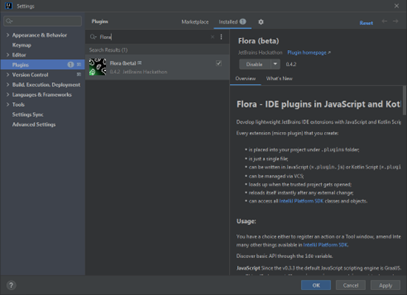
\includegraphics[width=.95\textwidth]{flora_plugin}}
    \caption{Flora Plugin im IntelliJ Plugin Marketplace.}
    \label{fig:FloraPlugin}
\end{figure}    
 
Das Plugin sucht dann in den geöffneten Projektverzeichnissen nach ausführbaren 
„micro plugin“-Dateien, die JavaScript oder Kotlin-Quellcode enthalten. 
Diese müssen sich in einem Ordner namens \emph{.plugins} 
befinden und auf \emph{.plugin.js}  oder \emph{.plugin.kts}  enden \cite{FloraPluginMarketplace}.
Innerhalb dieser Plugin-Dateien kann über die Variable \emph{ide} auf 
die angebotene Schnittstelle zugegriffen werden. Diese erlaubt 
es unter anderem Actions, Keyboard Shortcuts, Services und 
ToolWindows zu erstellen.

\begin{figure}
    \centering
    \fbox{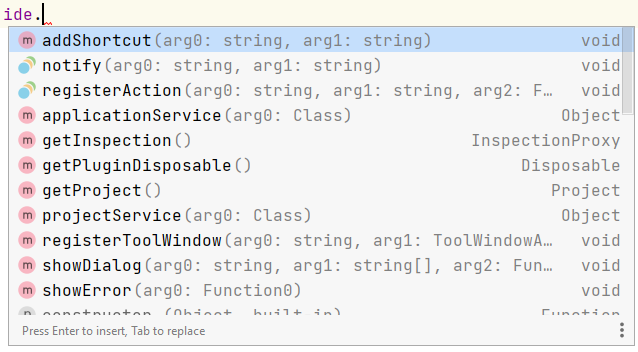
\includegraphics[width=.75\textwidth]{flora_codeCompletion}}
    \caption{Übersicht über die API des Flora Plugins.}
    \label{fig:FloraPluginAPI}
\end{figure}    
 
Flora Plugins bieten sich vor allem dann an, wenn eine projektspezifische 
Aufgabe automatisiert werden soll. Hier sind vor allem die 
Leichtgewichtigkeit der Plugins und die Schnelle, mit der ein 
einfaches Plugin entwickelt werden kann, von großem Vorteil. 
Weiters spricht für diesen Anwendungsfall, dass der Plugin Code 
direkt im Projektordner abgelegt wird und somit auch in einem Version 
Control System wie Git mit abgelegt werden kann.

% //TODO add references to subpages of docs

% //TODO fix manual \linebreak in multiple places 
\chapter{Anforderungen an den Prototyp}
\label{cha:Prototyp}

Für den direkten Vergleich der beiden Plugin APIs, sollte 
in VS Code und in IntelliJ ein möglichst funktionsgleicher 
Prototyp implementiert werden.

Durch diesen Prototyp können die Features der beiden APIs 
demonstriert und bewertet werden. Weiters bietet der Prototyp
eine praxisnahe Methode um sich auch mit dem Arbeitsablauf der
beiden Plattformen, speziell auch dem Veröffentlichen
des Plugins, vertraut zu machen.

\section{Aufbau}
\label{sec:Prototyp_Aufbau}

Um diese Aufgaben möglichst gut zu erfüllen, wurde das
\enquote{RecentChangesPlugin} entworfen. Kurz gesagt handelt
es sich dabei um ein Plugin, welches Text- oder Codeänderungen 
im Editor mitschreibt und die Wiederholung von gleichen oder
ähnlichen Änderungen erleichtert.
Als Änderung wird hierbei das einfache Abändern oder das Ersetzen eines
Wortes durch ein anderes verstanden. 
Das Mitschreiben von komplexeren Veränderungen, zum Beispiel 
wenn in mehreren Zeilen gleichzeitig Änderungen vorgenommen 
werden, ist nicht Ziel des Prototypen,da dies das Erkennen 
und das Wiederholen der Änderung stark verkomplizieren würde.

\subsection{Bemerken von Textänderungen}

Der Prototyp soll Änderungen in Text- oder Codedateien automatisch
erkennen können um diese mitzuschreiben. Hierfür muss auch erkannt
werden, wann eine Änderung vollständig abgeschlossen ist. Hierfür
soll ein Debounce-Effekt % //TODO cite
genutzt werden. Die erkannten Änderungen 
müssen analysiert und zwischengespeichert werden.

\subsection{Anwenden von Änderungen auf Befehl}

Der Prototyp soll zuvor erkannte Änderungen auf Befehl an der
aktuellen Position im Editor anwenden können. Dafür muss zuerst die
aktuelle Textcursor-Position analysiert werden, um das Wort zu finden,
an dem sich der Textcursor befindet. Danach muss in den 
zwischengespeicherten Änderungen ein passender Eintrag gefunden werden,
der auch auf die aktuelle Position angewendet werden kann.
Dabei sollen neuere Änderungen gegenüber älteren bevorzugt werden.

\subsection{Anwenden von Änderungen durch Tastenkombination}

Der Vorgang des Anwenden von Änderungen soll auch durch eine
Tastenkombination auslößbar sein.

\subsection{Vergessen von alten Änderungen}

Um erkannte Änderungen nicht ewig im Zwischenspeicher zu halten,
soll nur eine bestimmte Menge gleichzeitig gespeichert werden 
können. Wird diese Menge überschritten, so soll die älteste Änderung
aus dem Zwischenspeicher entfernt, und somit \enquote{vergessen}, werden.

\subsection{Automatische Codevervollständigung}

Anhand der kürzlichen Änderungen sollen auch Vorschläge
in der Codevervollständigung angezeigt werden. Für diese
Vorschläge sind natürlich nur die bereits geänderten Worte
relevant, nicht die die in der Änderung ersetzt wurden.

\subsection{Anzeige der Änderungen}

Damit die NutzerInnen einen Überblick über die kürzlichen Änderungen
haben, sollen alle Änderungen die sich im Zwischenspeicher befinden
über eine View angezeigt werden können.

\subsection{Einstellungen}

Es soll möglich Einstellungen des Plugins festzulegen, welche
auch beim Schließen der Entwicklungsumgebunge persistent bleiben.

Es soll gespeichert werden:
\begin{itemize}
    \item wie viele Änderungen gleichzeitig im 
        Zwischenspeicher gehalten werden.
    \item welche Debounce Zeit für das erkennen 
        von Änderungen verwendet wird. 
\end{itemize}

\subsection{Tests}

Es soll eine kleine, demonstrative Menge von Unit- und Intergrationstests für
den Plugin Code geschrieben werden.
\include{chapters/entwicklungVsCode}
\chapter{Entwicklung des Prototpys für IntelliJ}
\label{cha:EntwicklungIntelliJ}

\section{Design}
\label{sec:EntwicklungIntelliJ_Design}

Das beschriebene Plugin setzt sich in IntelliJ 
durch die Komponenten zusammen,
die in Abbildung \ref{fig:diagram_IntelliJDesign-Simplified} 
abgebildet sind.

\begin{figure}
    \centering
    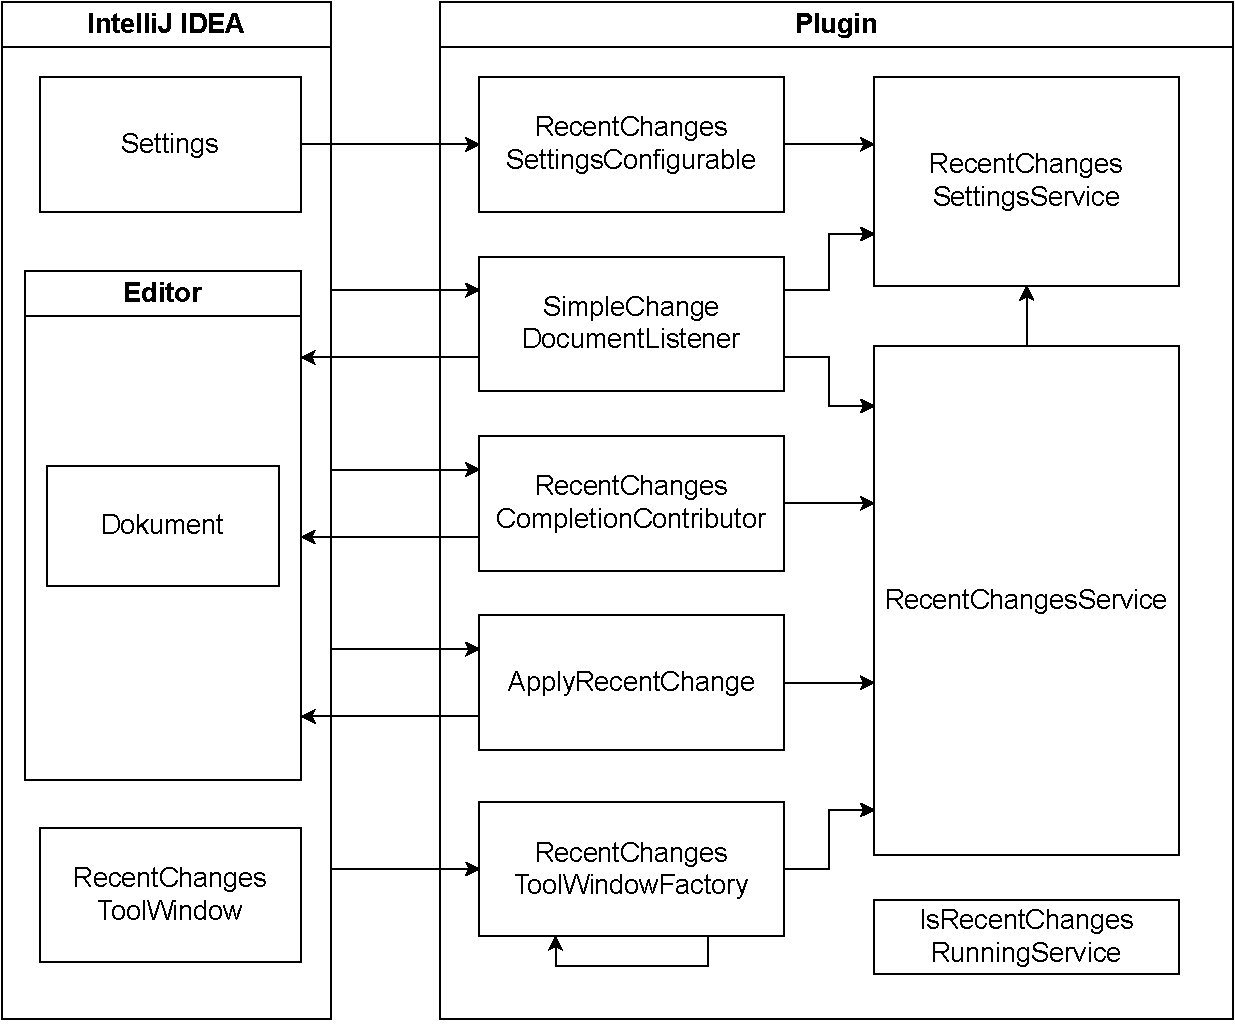
\includegraphics[width=.95\textwidth]{diagram_IntelliJDesign-Simplified}
    \caption{Vereinfachte Design-Übersicht des Plugins in IntelliJ.}
    \label{fig:diagram_IntelliJDesign-Simplified}
\end{figure}

Da die beiden Plugins im Aufbau sehr ähnlich sind, sind auch die Aufgaben der
Einzelnen Komponenten beinahe deckungsgleich. Die Unterschiede liegen eher in
den Details.

Der \emph{SimpleChangeDocumentListener} übernimmt hier die Aufgabe
des Beobachten des geöffneten Dokuments auf Veränderungen. Wird
eine Änderung festgestellt, so wird diese an den \emph{RecentChangesService}
zur Speicherung übergeben. Im Gegensatz zum \emph{RecentChangeStorage}
ist dieser allerdings als expliziter Service deklariert, der von IntelliJ
selbst verwaltet wird.

Die Komponenten für Einstellungen teilen sich auf 
\emph{RecentChangesSettingsConfigurable} und \emph{RecentChangesSettingsService}
auf. Die Klasse \emph{RecentChangesSettingsConfigurable} kümmert sich dabei
um die Darstellung und die Interaktivität der Einstellungen in der Benutzerschnittstelle.
Die Klasse \emph{RecentChangesSettingsService} wird wieder als Service 
angeboten und kümmert sich um das Speichern, Auslesen und Persistieren
der Einstellungen.

Die Codevervollständigung wird im IntelliJ Plugin durch den
\emph{RecentChangesCompletionContributor} durchgeführt. Dieser
sucht im \emph{RecentChangesService} nach Änderungen, die auf
das ausgewählte Wort passen und gibt diese als Vorschläge zurück.

Für das Einsetzen der Änderungen im Editor wird die Klasse
\emph{ApplyRecentChange} verwendet, die als Action registriert ist.
Bei der Action ist wie bereits im VS Code Plugin eine Tastenkombination
zum schnelleren Aufrufen hinterlegt.
Sollte keine passende Änderung gefunden werden, so wird direkt im
Editor ein Warnhinweis mit einer entsprechenden Meldung angezeigt.

% //TODO FIX manual \linebreak
Die Klasse \emph{RecentChangesToolWindowFactory} ist für die Darstellung
einer \linebreak
UI-Komponente zuständig, die dem TreeView aus dem VS Code Plugin
ähnelt. Sie liest dafür den Zustand des \emph{RecentChangesService} aus
und baut eine entsprechende Baumstruktur auf. Um die Ansicht auch zum richtigen
Zeitpunkt aktualisieren zu können, wird der Service mithilfe eines
Observer-Patterns \cite{2005Dp:e} beobachtet.

Die Komponente \emph{IsRecentChangesRunningService} existiert für den Fall,
das zwei Instanzen von IntelliJ gleichzeitig auf einem Gerät gestartet werden.
Beim Start der Anwendung müssen nämlich einige Initialisierungen vorgenommen
werden, die nur einmalig durchgeführt werden dürfen. Gegen den
\emph{IsRecentChangesRunningService} kann auf diese Weise geprüft werden, ob
die Initialisierung noch nötig ist oder bereits gemacht wurde.


\section{Implementierung}
\label{sec:EntwicklungIntelliJ_Implementierung}

\subsection{Aufsetzen des Projektes}

Das Erstellen eines neuen Plugin-Projektes kann in IntelliJ über den 
\enquote{New Project Wizard} erledigt werden
\cite{IntelliJPlatformSDKCreateProject}. Dafür muss einfach
im Programm IntelliJ IDEA das Menü \emph{File -> New -> Project...}
gewählt werden. Hier kann in der Liste der Projekt-Vorlagen
auch ein Eintrag für ein \emph{IDE Plugin}-Projekt gefunden werden.
Für diesen Projekttyp kann dann unter anderem
ein Name für das Projekt gewählt werden. Dieser Name wird initial auch als
Name des Plugins verwendet.

Die durch IntelliJ generierte Ordnerstruktur ist (ausschnittsweise) in 
Abbildung \ref{fig:intellij_generated_structure} dargestellt.
Relevant ist hier vor allem die Datei \emph{plugin.xml}, die das 
ent\-sprechend vorbereitete Plugin Manifest beinhaltet. Der Ordner
\emph{kotlin} ist als Verzeichnis für den Plugin-Code vorgesehen.
Für die Implementierung des \emph{RecentChangesPlugin} wurde dieser
allerdings durch einen Ordner \emph{java} ersetzt.
Ein Ordner für Tests wird nicht automatisch generiert
und muss manuell hinzugefügt werden.

\begin{figure}
    \centering
    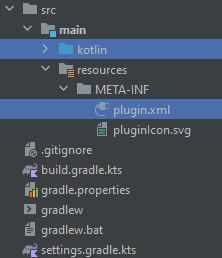
\includegraphics[width=.35\textwidth]{intellij_generated_structure}
    \caption{Ausschnitt der durch \emph{IntelliJ IDEA} generierten Ordnerstruktur.}
    \label{fig:intellij_generated_structure}
\end{figure}   

\subsection{Entwicklung}

\subsubsection{RecentChangesService}

Die Klasse \emph{RecentChangesService} (dargestellt in
Abbildung \ref{fig:diagram_IntelliJDesign-Detail_Service}) 
wird in der Form eines
Services auf Applikationsebene implementiert. Dies wird 
über das Attribut \emph{@Service(Service.Level.APP)} festgelegt. 
Auf diese Weise kann eine Instanz der Klasse in der gesamten Anwendung
bereitgestellt werden. Die statische Methode \emph{getInstance}
abstrahiert dabei die Aufrufe der IntelliJ API, die nötig sind, um eine
Referenz auf diese Instanz zu erhalten. Genau wie im VS Code Plugin,
werden die Änderungen in einer \emph{EvictingQueue} von 
\emph{SimpleDiff}-Objekten gespeichert. Allerdings muss diese
Warteschlange hier nicht selbst implementiert werden, da es in
der Bibliothek \emph{Guava} von Google bereits eine 
Implementierung gibt \cite{GuavaGitHub}.
Diese Bibliothek kann 
in der Datei \emph{build.gradle.kts} eingebunden werden.
Die verschiedenen Methoden der Klasse \emph{RecentChangesService} erlauben
das Einfügen sowie das Auslesen von \emph{SimpleDiff}-Objekten aus
der darunterliegenden Datenstruktur. Über die Methoden \emph{addChangeListener},
\emph{removeChangeListener} und \emph{notifyListeners} wird ein Observer-Pattern
abgebildet. Observer, welche die eigens erstellte Schnittstelle 
\emph{RecentDiffsChangedListener} implementieren, können sich also
beim \emph{RecentChangesService} anmelden. Sie werden dann bei Änderungen 
an den Daten über die Methode \emph{notifyChanged} notifiziert.
Da es sich bei der Klasse \emph{RecentChangesService} aufgrund der Implementierung
als IntelliJ Service um eine Singleton-Klasse \cite{2005Dp:e}
handelt, wird zusätzlich eine Methode \emph{reset} benötigt, um beim Testen
die Unabhängigkeit der verschiedenen Unit-Tests zu erhalten. Da für
die einzelnen Testfälle keine neuen Instanzen erzeugt werden können, muss
die Klasse also vor jedem Test zurückgesetzt werden.

\begin{figure}
    \centering
    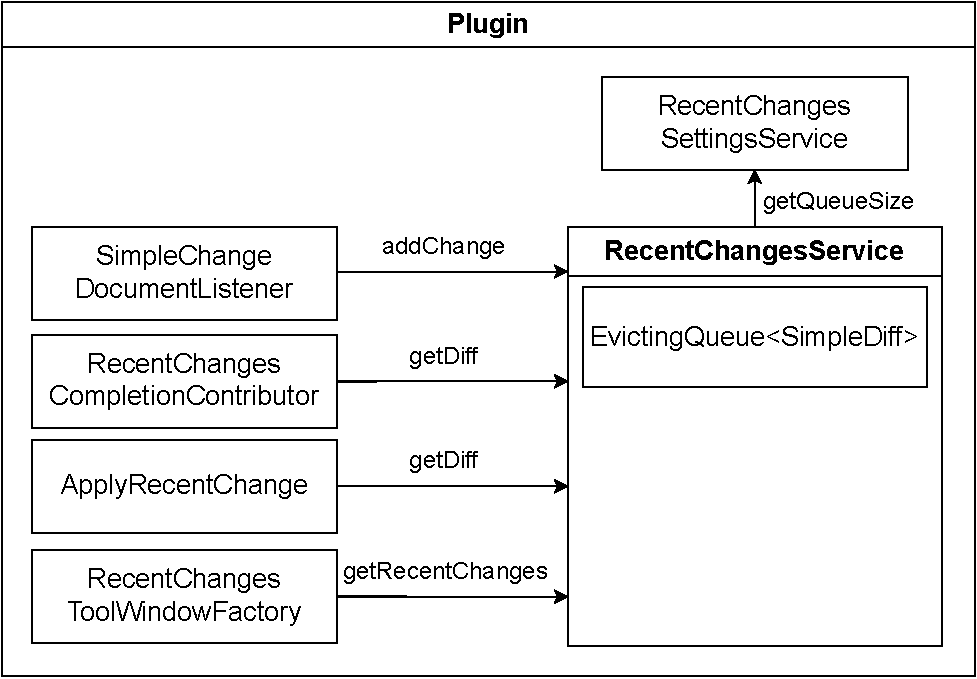
\includegraphics[width=.95\textwidth]{diagram_IntelliJDesign-Detail_Service}
    \caption{Detaillierte Darstellung des \emph{RecentChangesService}.}
    \label{fig:diagram_IntelliJDesign-Detail_Service}
\end{figure}

\subsubsection{SimpleChangeDocumentListener}

Der detaillierte Aufbau der Komponente \emph{SimpleChangeDocumentListener}
kann in Abbildung \ref{fig:diagram_IntelliJDesign-Detail_Listener} betrachtet werden.
Eine Instanz der Klasse wird beim ersten Start von IntelliJ so registriert, 
dass er über die Änderungen in \emph{allen} geöffneten Dokumenten informiert wird. 
Hierfür muss die Schnittstelle \emph{DocumentListener} implementiert werden.
Diese definiert unter anderem die Methodensignaturen \emph{beforeDocumentChange}
und \emph{documentChanged}. Durch das Zusammenspiel dieser beiden Methoden
wird der gewünschte Debounce-Effekt erzeugt. Zu Beginn einer Änderung
wird in der Methode \emph{beforeDocumentChange} der aktuelle Text aus der 
unveränderten Datei ausgelesen. In der Methode \emph{documentChanged} wird
dann ein Timer gestartet (oder neu gestartet, falls er bereits laufen sollte).
Erst nach Ablauf des Timers (ohne eine weitere Eingabe) wird
eine Änderung als abgeschlossen erkannt. Sobald dies geschieht, wird 
der Algorithmus \emph{diff-match-patch} verwendet, um die Änderung zu analysieren.
Wird daraufhin festgestellt, dass es sich um eine einfache Änderung handelt,
so wird diese in den Speicher des \emph{RecentChangesService} eingefügt.
Zu beachten ist in dieser Klasse weiters die private Methode 
\emph{getOriginalTextFromDocument}. Dieser komplexe Aufruf % //TODO rewrite after call is simplified, //TODO simplify code
ist in IntelliJ notwendig, um den reinen Text des veränderten Dokuments
zu erhalten. Die Klasse \emph{Document} hätte zwar eigentlich
eine Methode \emph{getText}, dieser Text befindet sich aber möglicherweise
in einem Zwischenzustand, in dem IntelliJ spezielle Zeichenketten 
einsetzt, um die Anzeige der Codevervollständigung zu erleichtern
\cite{IntelliJTheDreadedString,IntelliJGitHubCompletionUtilCore}.
Um die originale Datei (und nicht eine modifizierte Kopie) zu erhalten,
müssen also einige Umwege gegangen werden. % //TODO fix: weird page break in pdf. werden is on the next page.

\begin{figure}
    \centering
    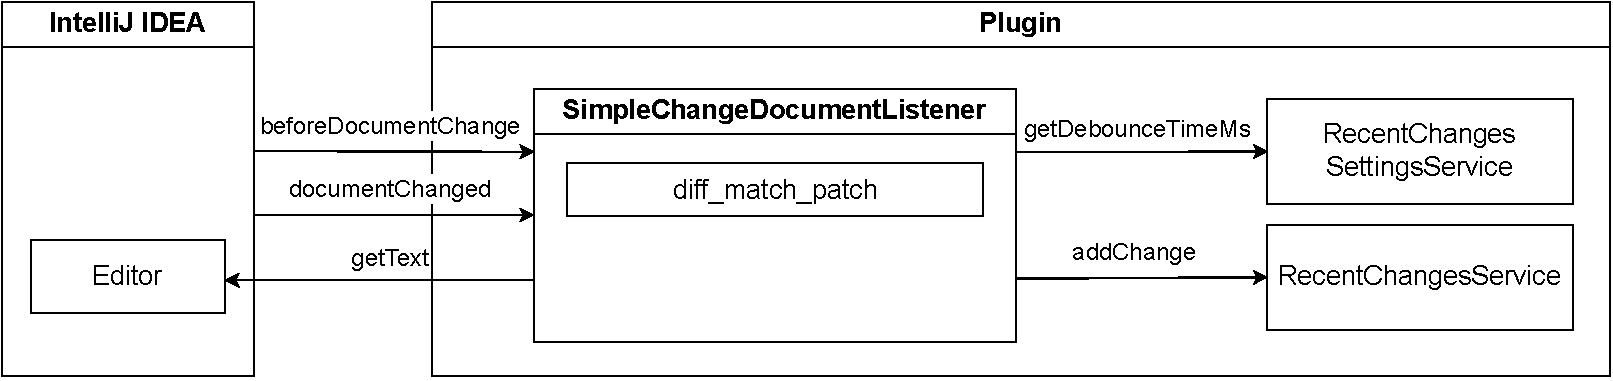
\includegraphics[width=.95\textwidth]{diagram_IntelliJDesign-Detail_Listener}
    \caption{Detaillierte Darstellung des \emph{SimpleChangeDocumentListener}.}
    \label{fig:diagram_IntelliJDesign-Detail_Listener}
\end{figure}

\subsubsection{ApplyRecentChange}

Bei \emph{ApplyRecentChange} handelt es sich um eine von
\emph{AnAction} abgeleitete Klasse. In Abbildung
\ref{fig:diagram_IntelliJDesign-Detail_Action} sind die Interaktionen
der Klasse dargestellt. Die Methoden \emph{actionPerformed} und \emph{update}
werden von IntelliJ aufgerufen. In beiden Methoden muss zuerst
der Inhalt der Datei an der aktuellen Position gelesen werden, um 
herauszufinden, ob das Anwenden der Action momentan möglich ist.
Sollte das Anwenden nicht möglich sein, wird
in der Methode \emph{update} mithilfe des übergebenen
\emph{AnActionEvent}-Objekt die Sichtbarkeit der Action (in den
registrierten Menüs des User Interface) gesetzt.
In der Methode \emph{actionPerformed} wird in einem solchen Fall
eine Fehlermeldung mithilfe des IntelliJ Services \emph{HintManager}
angezeigt. Sollte ein Ersetzen möglich sein,
so wird mittels der statischen Methode 
\emph{WriteCommandAction.runWriteCommandAction} ein Schreibbefehl
abgesetzt, in welchem der zu ersetzende Inhalt des Dokuments 
ausgetauscht wird. Dies ist nur über einen solchen Schreibbefehl möglich,
da ansonsten Synchronisationsprobleme auftreten könnten
\cite{IntelliJPlatformSDKSafelyReplacingText,IntelliJPlatformSDKGeneralThreadingRules}.
Im Manifest des Plugins wird die Action mit der 
Tastenkombination \emph{alt + R} registriert, um
auch Aufrufbar zu sein.

\begin{figure}
    \centering
    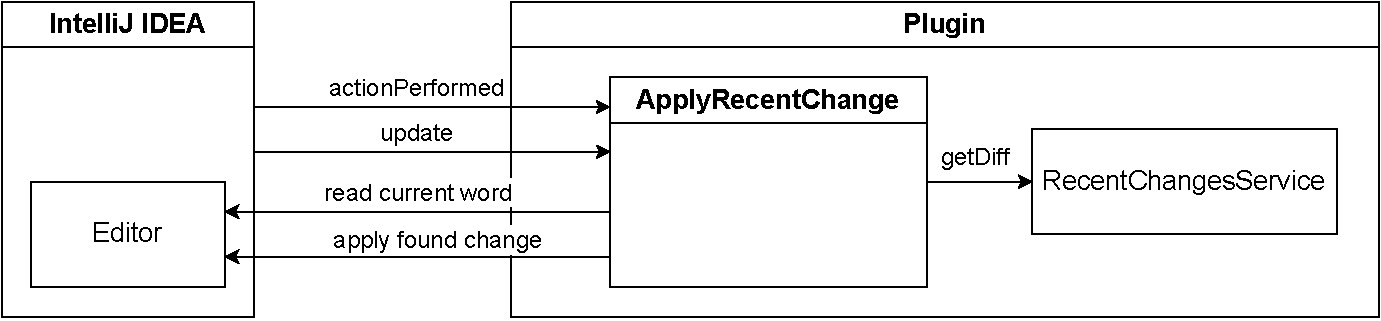
\includegraphics[width=.95\textwidth]{diagram_IntelliJDesign-Detail_Action}
    \caption{Detaillierte Darstellung der Action \emph{ApplyRecentChange}.}
    \label{fig:diagram_IntelliJDesign-Detail_Action}
\end{figure}

\subsubsection{RecentChangesCompletionContributor}

Die Klasse \emph{RecentChangesCompletionContributor}, die in Abbildung
\ref{fig:diagram_IntelliJDesign-Detail_Contributor} dargestellt wird,
leitet von \emph{CompletionContributor} ab. Im Konstruktor muss
die Methode \emph{extend} aufgerufen werden, der eine Instanz 
des eigentlichen \emph{CompletionProvider} übergeben wird.
Dieser \emph{CompletionProvider} überschreibt wiederum die 
Methode \emph{addCompletions}, welche die eigentliche Arbeit erledigt.
Genau wie bei der Action \emph{ApplyRecentChange}, wird der
Inhalt der Datei an der aktuellen Position ausgelesen. Das gefundene
Wort wird im \emph{RecentChangesService} nachgeschlagen.
Falls eine passende Änderung gefunden wird, wird diese über den 
Parameter \emph{resultSet} zu den Vorschlägen für die Codevervollständigung
hinzugefügt.
Im Manifest wird der Contributor für die Sprache \emph{any} registriert,
um sprachunabhängig zu funktionieren.

\begin{figure}
    \centering
    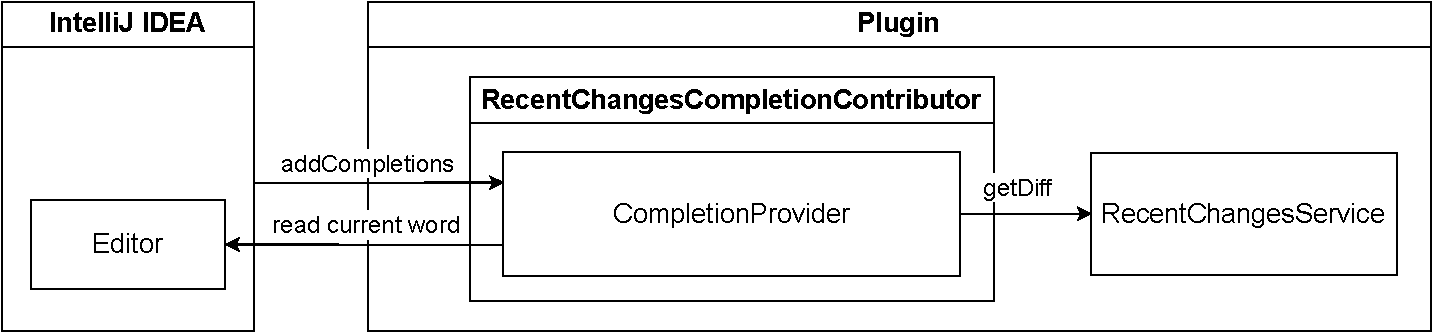
\includegraphics[width=.95\textwidth]{diagram_IntelliJDesign-Detail_Contributor}
    \caption{Detaillierte Darstellung des \emph{RecentChangesCompletionContributor}.}
    \label{fig:diagram_IntelliJDesign-Detail_Contributor}
\end{figure}

\subsubsection{RecentChangesToolWindowFactory}

Die Klasse \emph{RecentChangesToolWindowFactory} ist in Abbildung
\ref{fig:diagram_IntelliJDesign-Detail_ToolWindow} dargestellt.
Sie implementiert die Schnittstelle \emph{ToolWindowFactory} 
und überschreibt die Methode \emph{createToolWindowContent}. Zur besseren 
Abgrenzung der Aufgaben wird in dieser zuerst eine neue Instanz
der Klasse \emph{RecentChangesToolWindowContent} erstellt.
Diese innere Klasse verwaltet den Inhalt und das Aussehen des Fensters.
Sie lädt die nötigen Daten aus dem \emph{RecentChangesService} und
meldet sich bei dem Service auch als Listener an, um gegebenenfalls den
Inhalt zu aktualisieren. Die Darstellung des Fensterinhalts
geschieht über ein \emph{JPanel} aus Java Swing und einem \emph{Tree}
aus der UI-Bibliothek von IntelliJ. Dieser Inhalt wird
durch die Methode \emph{getContentPanel} von außen zugänglich gemacht.
Zum Schluss setzt die Methode \emph{createToolWindowContent} 
den eigentlichen Inhalt des Fensters durch den Aufruf von
\emph{toolWindow.getContentManager().addContent} auf dem übergebenen
Parameter.
Im Manifest wird \emph{RecentChangesToolWindowFactory} als Factory-Klasse
für ein ToolWindow namens \emph{Recent Changes} registriert.

\begin{figure}
    \centering
    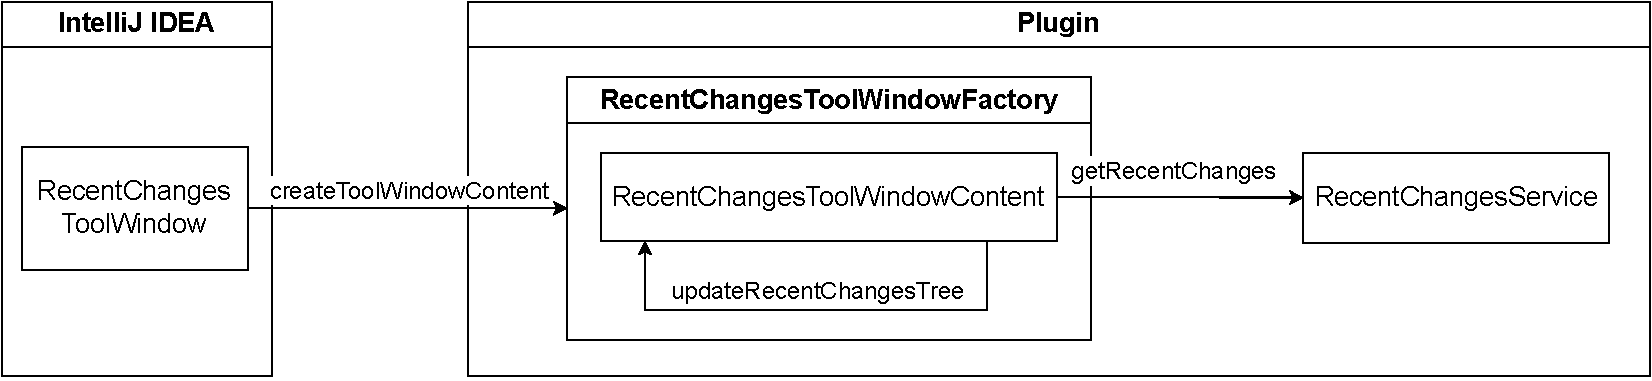
\includegraphics[width=.95\textwidth]{diagram_IntelliJDesign-Detail_ToolWindow}
    \caption{Detaillierte Darstellung der \emph{RecentChangesToolWindowFactory}.}
    \label{fig:diagram_IntelliJDesign-Detail_ToolWindow}
\end{figure}

\subsubsection{Einstellungen}

Die für die Einstellungen nötigen Klassen sind in Abbildung
\ref{fig:diagram_IntelliJDesign-Detail_Settings} zu sehen.
\emph{RecentChangesSettingsConfigurable} ist die Hauptschnittstelle 
zu IntelliJ, die auch im Manifest registriert ist. 
Sie implementiert das Interface \emph{Configurable}
und bietet verschiedene Methoden an, die für die Darstellung
und Interaktivität in der Benutzerschnittstelle nötig sind.
Durch die Methode \emph{apply} sollen die aktuell gewählten Einstellungen
persistiert werden, durch die Methode \emph{reset} die 
zuvor gespeicherten Einstellungen wieder angezeigt werden.
Durch die Methode \emph{isModified} wird überprüft, ob die angezeigten
Einstellungen von den persistierten Einstellungen abweichen. 
Ist dies nicht der Fall, wird der Knopf zum Speichern der Einstellungen
automatisch ausgegraut. Die Methode \emph{createComponent} stellt
den Inhalt der Einstellungsseite in Form eines \emph{JComponent} bereit.
Um gute Aufgabenteilung zu ermöglichen, ist diese Darstellung an die 
Klasse \emph{RecentChangesSettingsComponent} ausgelagert. Sie beinhaltet
Felder zum Eingeben der Warteschlangengröße und der Debouncezeit.
Über Getter- und Setter-Methoden können diese Werte von 
\emph{RecentChangesSettingsConfigurable} beliebig verwaltet werden.
Um das Eingeben von ungültigen Werten zu vermeiden, werden zusätzlich
Filter auf die Eingabefelder angewandt.
Der \emph{RecentChangesSettingsService} ist die Komponente die für das 
Persistieren der Einstellungen verantwortlich ist. Hierfür
wird die Schnittstelle \emph{PersistentStateComponent} implementiert
und das Attribut \emph{@State} angegeben. Auf diese Weise ruft
IntelliJ zu den passenden Zeitpunkten automatisch die Methoden
\emph{getState} und \emph{loadState} auf und serialisiert den Zustand
in einer \emph{.xml}-Datei.
Zusätzlich ist die Klasse im Manifest als Service registriert, und bietet
passende Methoden zum Auslesen und Setzen sowie ein Observer-Pattern
zum Beobachten der Einstellungen an.

\begin{figure}
    \centering
    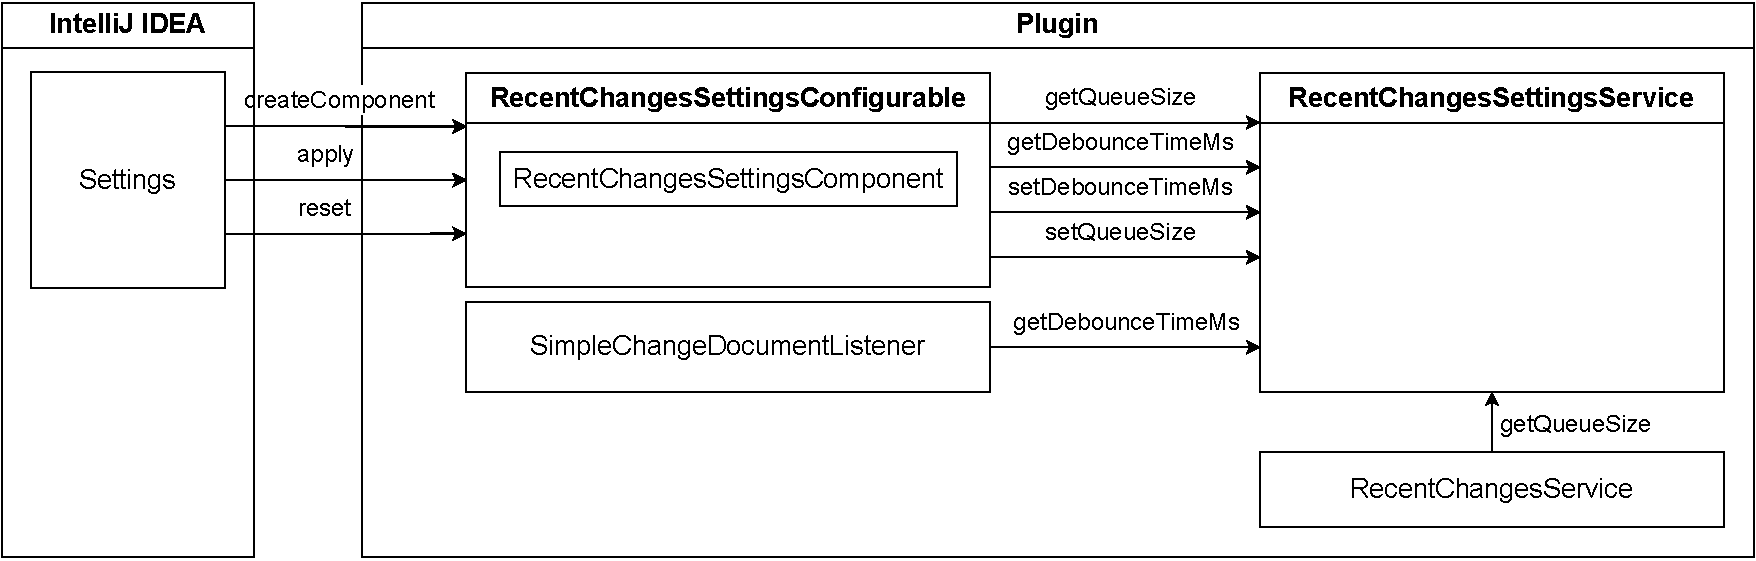
\includegraphics[width=.95\textwidth]{diagram_IntelliJDesign-Detail_Settings}
    \caption{Detaillierte Darstellung der \emph{Settings} Komponenten.}
    \label{fig:diagram_IntelliJDesign-Detail_Settings}
\end{figure}

\section{Tests}
\label{sec:EntwicklungIntelliJ_Tests}

Für Tests eines IntelliJ-Plugins werden von JetBrains 
die Frameworks \emph{JUnit}, \emph{TestNG} und \emph{Cucumber} empfohlen
\cite{IntelliJPlatformSDKTestsAndFixtures}. 
Alle Tests für das IntelliJ Plugin laufen innerhalb einer sogenannten
\emph{headless Umgebung} \cite{IntelliJPlatformSDKTestingOverview}. 
Das bedeutet, es wird eine echte Instanz
des IntelliJ IDEA zum Testen verwendet. Dieses wird allerdings ohne einer
Benutzerschnittstelle gestartet und wird daher nicht angezeigt.
Als Hauptschnittstelle für die Tests bietet IntelliJ die Klassen
\emph{BasePlatformTestCase} und \emph{HeavyPlatformTestCase}
\cite{IntelliJPlatformSDKLightAndHeavyTests}.
Bei Test-Klassen, die von \emph{HeavyPlatformTestCase} ableiten,
handelt es sich um \emph{Heavy}-Tests. Diese erstellen in
der Testumgebung für jeden Testfall ein neues (temporäres)
Projekt, in welchem das Plugin arbeiten kann. Da das Erstellen solcher
Projekte allerdings sehr aufwändig ist, führt das Einsetzen solcher
Tests zu längeren Ausführungszeiten.
Bei Test-Klassen, die von \emph{BasePlatformTestCase} ableiten,
handelt es sich um \emph{Light}-Tests. Diese sind darauf optimiert,
möglichst effizient abzulaufen und versuchen, wenn möglich, das 
erstellte Projekt von vorherigen Tests weiter zu verwenden.
Dadurch wird zwar an Geschwindigkeit gewonnen, allerdings
muss speziell darauf geachtet werden, dass keine Abhängigkeiten zwischen
den Testfällen entstehen.
Sollten diese beiden Klassen zu einschränkend sein, kann auch die
Klasse \emph{IdeaTestFixtureFactory} verwendet werden
\cite{IntelliJPlatformSDKTestsAndFixtures}. Mit dieser
müssen allerdings einige \emph{setup}-Methoden manuell aufgerufen
werden und man hat einen höheren Konfigurationsaufwand.
Innerhalb der Testfälle kann beliebig mit der IntelliJ API interagiert
werden. Es gibt sogar zusätzliche Methoden wie \emph{copyFileToProject},
\emph{type}, \emph{performEditorAction}
\cite{IntelliJPlatformSDKTestProjectAndTestdataDirectories,IntelliJPlatformSDKWritingTests}. 
Diese erleichtern das Arbeiten mit der headless Umgebung 
und erlauben es zum Beispiel, Tastatureingaben zu simulieren.
Wenn Dateien in das Testprojekt geladen werden, kann spezielles Markup
verwendet werden. So kann beispielsweise mit \emph{<caret>} die Position
markiert werden, an der sich der Cursor befinden soll.

\section{Publishing}
\label{sec:EntwicklungIntelliJ_Publishing}

Um ein Plugin in IntelliJ zu veröffentlichen, gibt es mehrere Voraussetzungen
\cite{IntelliJPlatformSDKPluginSigning}.
Man benötigt einen Account im JetBrains Marketplace und ein Zertifikat
zum Signieren des Plugins. Der Account kann über die Seite 
\url{https://plugins.jetbrains.com/} erstellt werden. Das Generieren eines
Zertifikats und den dafür benötigten Schlüsseln geht mithilfe des 
Programms \emph{openssl} und ist in der IntelliJ Dokumentation beschrieben.

Im ersten Schritt muss das Plugin gebaut werden. Dies ist über den
Gradle Task \emph{buildPlugin} möglich, welcher das Plugin baut, und
das Ergebnis im Ordner \emph{build/distributions} als \emph{.zip}-Datei
speichert.

Um das gebaute Plugin zu signieren, können die im Projekt bereits vordefinierten
Gradle Tasks genutzt werden. Hierfür muss allerdings die Datei 
\emph{build.gradle.kts} angepasst werden. Im Abschnit \emph{signPlugin}
müssen das zuvor generierte Zertifikat, der dazugehörige Privatschlüssel
und das Passwort, mit welchem der Schüssel erstellt wurde, angegeben werden.
Um diese sensiblen Daten nicht unabsichtlich zu veröffentlichen, empfiehlt
es sich hier auf Umgebungsvariablen des Systems zurückzugreifen, welche
natürlich entsprechend gesetzt werden müssen.
\begin{JsCode}[numbers=none]
    signPlugin {
        certificateChain.set(System.getenv("IJ_PluginSign_CertChain"))
        privateKey.set(System.getenv("IJ_PluginSign_PK"))
        password.set(System.getenv("IJ_PluginSign_Pass"))
    }
\end{JsCode}
Durch Ausführung des Task \emph{signPlugin} kann das Plugin signiert werden.

Nach dem Signieren kann das Plugin veröffentlicht werden
\cite{IntelliJPlatformSDKPublishingAPlugin}.
Das Hochladen des Plugins in den JetBrains Marketplace muss beim ersten Mal
manuell gemacht werden. Hierfür meldet man sich auf der Webseite an,
klickt am oberen rechten Rand auf seinen Benutzernamen und daraufhin
auf \emph{Upload plugin}. Im erscheinenden Dialog gibt man
danach die nötigen Daten ein und lädt die zuvor generierte und signierte
\emph{.zip}-Datei hoch.
Das hochgeladene Plugin kann dann auf der Seite des eigenen Profils
verwaltet und mit zusätzlichen Informationen, wie zum Beispiel Screenshots,
ausgeschmückt werden.
Bevor das Plugin öffentlich im Marketplace angeboten wird, wird es 
zusätzlich von JetBrains Mitarbeitern geprüft. Um diese Prüfung
zu bestehen, sollte bereits vor dem Hochladen auf verschiedene
Anforderungen geachtet werden, die in der Dokumentation beschrieben sind.
So muss zum Beispiel beachtet werden, was als Logo verwendet wird, welcher
Titel gewählt wurde und wie die Beschreibung formatiert ist.
Diese Richtlinien können unter \url{https://plugins.jetbrains.com/docs/marketplace/plugin-overview-page.html}
nachgeschlagen werden.

Laut der IntelliJ Dokumentation ist es auch möglich ein
Plugin automatisiert in den Marketplace hochzuladen. Hierfür
kann der Gradle Task \emph{publishPlugin} in Kombination
mit einem Access Token von der Marketplace Webseite genutzt werden.
Dieser muss wiederum in der Datei \emph{build.gradle.kts} gesetzt werden.
\begin{JsCode}[numbers=none]
    publishPlugin {
        token.set(System.getenv("IJ_PluginSign_PublishToken"))
    }
\end{JsCode}
% //TODO publish fails
% documented issue: https://github.com/JetBrains/gradle-intellij-plugin/issues/870
% documented issue: https://github.com/JetBrains/gradle-intellij-plugin/issues/1482

\section{CI/CD}
\label{sec:EntwicklungIntelliJ_CICD}

Für das automatisierte Testen und Veröffentlichen eines Plugins
gibt es einen vorgefertigten GitHub Actions Workflow für 
Plugin-Projekte, die mit Gradle arbeiten \cite{IntelliJGitHubBuildWorkflow}.
Für andere CI/CD Pipelines gibt es keine Dokumentation.

Die Pipeline muss im Grunde verschiedene vordefinierte Gradle Tasks
ausführen. Das Ausführen der Tests ist beispielsweise durch den Befehl
\begin{GenericCode}[numbers=none]
    ./gradlew check
\end{GenericCode}
möglich. Das Veröffentlichen des Plugins kann durch
\begin{GenericCode}[numbers=none]
    ./gradlew publishPlugin 
\end{GenericCode}
angestoßen werden. 
% //TODO see if problems still arise or may be fixed somehow...
% Beim Veröffentlichen treten allerdings die
% selben Probleme auf, wie sie in Abschnitt \ref{sec:EntwicklungIntelliJ_Publishing}
% beschrieben sind.
\chapter{Bewertungskriterien}
\label{cha:Kriterien}


% \begin{description}
%     \item[Popularität der Entwicklungsumgebung] 
%     \label{sec:Kriterien_Popularität}    
%     Die Popularität von VS Code und IntelliJ kann aufgrund
%     von verschiedenen Umfragen und beliebtheits-Indizes 
%     analysiert werden. Dabei darf allerdings nicht außer
%     Acht gelassen werden, dass es sich bei VS Code und
%     IntelliJ nicht zwingend um Konkurrenzprodukte handelt,
%     sondern die beiden IDEs unterschiedliche Zielgruppen ansprechen.
%     Natürlich ist auch zu beachten wie viele Plugins 
%     für die Entwicklungsumgebung existieren, und somit wie 
%     populär die Entwicklungsumgebung bei Plugin EntwicklerInnen ist. 

%     Die Popularität von VS Code und IntelliJ kann aufgrund
%     von verschiedenen Umfragen und beliebtheits-Indizes 
%     analysiert werden. Dabei darf allerdings nicht außer
%     Acht gelassen werden, dass es sich bei VS Code und
%     IntelliJ nicht zwingend um Konkurrenzprodukte handelt,
%     sondern die beiden IDEs unterschiedliche Zielgruppen ansprechen.
%     Natürlich ist auch zu beachten wie viele Plugins 
%     für die Entwicklungsumgebung existieren, und somit wie 
%     populär die Entwicklungsumgebung bei Plugin EntwicklerInnen ist. 

%     \item[Performance] 
%     \label{sec:Kriterien_Performance}    
%     Da es sich bei den IDEs um komplexe Systeme handelt und die 
%     entwickelten Plugins sehr eng mit diesen Systemen verwoben sind,
%     ist es nur schwer möglich die Performance der entwickelten
%     Plugins zu vergleichen. Allerdings kann die allgemeine
%     Performance der IDEs verglichen werden.

%     \item[Feature Umfang] 
%     \label{sec:Kriterien_FeatureUmfang}    
%     Hier soll verglichen werden, wie viele Funktionen
%     den EntwicklerInnen von den Plugin APIs 
%     bereits zur Verfügung gestellt werden.

%     \item[Intuitivität der API] 
%     \label{sec:Kriterien_Intuitivität}    
%     Die Intuitivität der Plugin APIs kann bewertet werden,
%     in dem verglichen wird, wie einfach es ist die
%     angebotenen Features zu verwenden.
%     Dabei muss unter anderem beachtet werden wie viel Vorwissen über die
%     API man mitbringen muss, wie viele Abhängigkeiten es
%     gibt die nicht von Anfang an klar sind und ob es 
%     häufige Fallstricke gibt, die EntwicklerInnen vermeiden müssen.

%     \item[Dokumentation der API] 
%     \label{sec:Kriterien_Dokumentation}    
%     Um eine Plugin API zu erlernen dient als erste Grundlage
%     immer die Dokumentation. Hier muss vor allem
%     auf Übersichtlichkeit und Vollstädingkeit großer Wert
%     gelegt werden.

%     \item[Testbarkeit des Plugins] 
%     \label{sec:Kriterien_Testbarkeit}    
%     Automatisierte Softwaretests zählen zu den wichtigsten
%      Standards in der Softwareentwicklung.
%     Um sicherzustellen, dass NutzerInnen eine gute User Experience
%     geboten wird, müssen die Plugin APIs das Testen der
%     Plugins nicht nur ermöglichen sondern möglichst
%     gut unterstützen.

%     \item[Möglichkeiten des Publishings] 
%     \label{sec:Kriterien_Publishing}    
%     Hier soll vorallem betrachtet werden, wie
%     einfach es für EntwicklerInnen ist ein Plugin zu 
%     veröffentlichen, aber auch welche Möglichkeiten es gibt 
%     das Plugin zu Vermarkten. Dabei ist nicht nur die Möglichkeit
%     auf Monetarisierung relevant, sondern auch die
%     Optionen für die Darstellung des Plugins im Marketplace 
%     (zum Beispiel die Einbindung von Logos oder Beschreibungstexten)

%     \item[Installationsprozess des Plugins] 
%     \label{sec:Kriterien_Installationsprozess}    
%     Zuletzt ist auch wichtig wie leicht es für potentielle 
%     NutzerInnen ist, das entwickelte Plugin zu finden und
%     in ihrer Programmierumgebung zu installieren.

% \end{description}

\section{Popularität der Entwicklungsumgebung}
\label{sec:Kriterien_Popularität}
Die Popularität von VS Code und IntelliJ kann aufgrund
von verschiedenen Umfragen und beliebtheits-Indizes 
analysiert werden. Dabei darf allerdings nicht außer
Acht gelassen werden, dass es sich bei VS Code und
IntelliJ nicht zwingend um Konkurrenzprodukte handelt,
sondern die beiden IDEs unterschiedliche Zielgruppen ansprechen.
Natürlich ist auch zu beachten wie viele Plugins 
für die Entwicklungsumgebung existieren, und somit wie 
populär die Entwicklungsumgebung bei Plugin EntwicklerInnen ist. 

Die Popularität von VS Code und IntelliJ kann aufgrund
von verschiedenen Umfragen und beliebtheits-Indizes 
analysiert werden. Dabei darf allerdings nicht außer
Acht gelassen werden, dass es sich bei VS Code und
IntelliJ nicht zwingend um Konkurrenzprodukte handelt,
sondern die beiden IDEs unterschiedliche Zielgruppen ansprechen.
Natürlich ist auch zu beachten wie viele Plugins 
für die Entwicklungsumgebung existieren, und somit wie 
populär die Entwicklungsumgebung bei Plugin EntwicklerInnen ist. 


\section{Performance}
\label{sec:Kriterien_Performance}

Da es sich bei den IDEs um komplexe Systeme handelt und die 
entwickelten Plugins sehr eng mit diesen Systemen verwoben sind,
ist es nur schwer möglich die Performance der entwickelten
Plugins zu vergleichen. Allerdings kann die allgemeine
Performance der IDEs verglichen werden.


\section{Feature Umfang}
\label{sec:Kriterien_FeatureUmfang}

Hier soll verglichen werden, wie viele Funktionen
den EntwicklerInnen von den Plugin APIs 
bereits zur Verfügung gestellt werden.


\section{Intuitivität der API}
\label{sec:Kriterien_Intuitivität}

Die Intuitivität der Plugin APIs kann bewertet werden,
in dem verglichen wird, wie einfach es ist die
angebotenen Features zu verwenden.
Dabei muss unter anderem beachtet werden wie viel Vorwissen über die
API man mitbringen muss, wie viele Abhängigkeiten es
gibt die nicht von Anfang an klar sind und ob es 
häufige Fallstricke gibt, die EntwicklerInnen vermeiden müssen.


\section{Dokumentation der API}
\label{sec:Kriterien_Dokumentation}

Um eine Plugin API zu erlernen dient als erste Grundlage
immer die Dokumentation. Hier muss vor allem
auf Übersichtlichkeit und Vollstädingkeit großer Wert
gelegt werden.


\section{Testbarkeit des Plugins}
\label{sec:Kriterien_Testbarkeit}

Automatisierte Softwaretests zählen zu den wichtigsten
Standards in der Softwareentwicklung.
Um sicherzustellen, dass NutzerInnen eine gute User Experience
geboten wird, müssen die Plugin APIs das Testen der
Plugins nicht nur ermöglichen sondern möglichst
gut unterstützen.


\section{Möglichkeiten des Publishings}
\label{sec:Kriterien_Publishing}

Hier soll vorallem betrachtet werden, wie
einfach es für EntwicklerInnen ist ein Plugin zu 
veröffentlichen, aber auch welche Möglichkeiten es gibt 
das Plugin zu Vermarkten. Dabei ist nicht nur die Möglichkeit
auf Monetarisierung relevant, sondern auch die
Optionen für die Darstellung des Plugins im Marketplace 
(zum Beispiel die Einbindung von Logos oder Beschreibungstexten)


\section{Installationsprozess des Plugins}
\label{sec:Kriterien_Installationsprozess}

Zuletzt ist auch wichtig wie leicht es für potentielle 
NutzerInnen ist, das entwickelte Plugin zu finden und
in ihrer Programmierumgebung zu installieren.
\chapter{Vergleich anhand der Bewertungskriterien}
\label{cha:Vergleich}

\section{Popularität der Entwicklungsumgebung}
\label{sec:Vergleich_Popularität}

\subsection{Visual Studio Code}

Laut der Stack Overflow Developer Survey von 2023 ist
VS Code der große Spitzenreiter der IDEs. Es wurde von
73,71\% der EntwicklerInnen angegeben,
dass sie VS Code verwenden \cite{StackOverflowSurvey2023}.
Auch der PYPL Index bestätigt die Beliebtheit von VS Code~\cite{PYPL}.
Dieser Index misst die Anzahl von Suchanfragen in der Google Suchmaschine
und reiht VS Code auf den zweiten Platz hinter Visual Studio.

Die Anzahl von Extensions, die im Visual Studio Marketplace angeboten werden,
beträgt aktuell über 54.000 \cite{VSCodeMarketplace}. Allerdings sind 
darunter auch viele Extensions, die kaum verwendet werden und die nur
wenige Downloads vorweisen können. Zählt man nur die 
Extensions, die über eine Million Downloads erreicht haben,
kommt man auf etwas über 350 Extensions.

\subsection{IntelliJ IDEA}

In der Stack Overflow Developer Survey gaben 2023
26,42\% der EntwicklerInnen an, IntelliJ IDEA zu verwenden,
womit es in der Umfrage den dritten Platz erreichte~\cite{StackOverflowSurvey2023}.
PYPL stuft IntelliJ auf Platz sieben ihres Index ein \cite{PYPL}.
Allerdings darf hierbei nicht vergessen werden, dass Plugins
für die IntelliJ Platform auch in anderen JetBrains IDEs installiert
werden können. Berechnet man aus den Daten der Stack Overflow Umfrage
eine gemeinsame Beliebtheit der IntelliJ Platform IDEs, so findet man,
dass 52,87\% der EntwicklerInnen eine solche Programmierumgebung nutzen \cite{StackOverflowSurvey}.
Weiters muss beachtet werden, dass die Zielgruppe von IntelliJ IDEA
vor allem Java EntwicklerInnen sind. Bei Umfragen mit Java-EntwicklerInnen 
schneidet IntelliJ IDEA meist mit dem ersten Platz ab \cite{JRebelIDEs,JRebelDeveloperProductivityReport,BetterprojectsfasterPouplarityIndex}.

Im JetBrains Marketplace werden für die gesamte IntelliJ Platform aktuell
etwas über 7.800 Plugins zum Download angeboten. Zählt man nur die 
Plugins mit mehr als einer Million Downloads, kommt man auf
knapp über 100 Plugins.

\subsection{Vergleich}

Während es sich bei VS Code um einen allgemeinen Code-Editor handelt,
der sehr vielseitig eingesetzt werden kann, bietet die IntelliJ-Plattform
eher spezifische Werkzeuge, die in erster Linie auf die Entwicklung in
einer einzelnen Programmiersprache ausgerichtet sind.
Obwohl VS Code zwar insgesamt der häufiger genutzte Editor ist,
sind die JetBrains IDEs für das Programmieren in einer 
speziellen Sprache (zum Beispiel IntelliJ IDEA für Java) oft die
beliebtere Wahl.
    

\section{Ausführungszeit und Hardwareanforderungen}
\label{sec:Vergleich_Performance}

\subsection{Visual Studio Code}

Mithilfe der Anwendung \emph{AppTimer} von PassMark wurde
die durchschnittliche Startzeit von VS Code ermittelt \cite{PassMarkAppTimer}.
AppTimer wurde so konfiguriert, dass VS Code automatisch gestartet
und wieder geschlossen wird. Beim Start wurde von VS Code ein
einfacher Projektordner geladen. Der AppTimer maß bei jedem Start
die Zeit die VS Code brauchte, um in einen Zustand zu gelangen,
in dem Nutzereingaben angenommen werden konnten.
Diese Messung wurde in 100 Iterationen wiederholt.
Daraus ergab sich eine durchschnittliche Startzeit von 0.294 Sekunden.

Die Hardwareanforderungen sind gering. VS Code benötigt weniger
als 500 MB Festplattenspeicher, 1 GB RAM und eine Prozessorgeschwindigkeit
von 1.6 GHz, um lauffähig zu sein.

\subsection{IntelliJ IDEA}

Die Messungen mithilfe der AppTimer-Anwendung wurden auch
für IntelliJ IDEA Ultimate in 100 Iterationen wiederholt.
Hier war die durchschnittliche Startzeit bei 8.123 Sekunden.

Für die Hardwareanforderungen gibt IntelliJ IDEA
mindestens 3.5 GB Festplattenspeicher, 2 GB RAM und eine
moderne CPU vor.

\subsection{Vergleich}

Da es sich bei VS Code nur um einen leichtgewichtigen Editor handelt,
hat dieser auch einen klaren Vorteil bei der Performance 
und den Hardwareanforderungen.
IntelliJ IDEA ist eine vollständige IDE und hat daher auch längere
Startzeiten und höhere Hardwareanforderungen.
Auf modernen Geräten sollten beide Entwicklungsumgebungen
problemlos ausführbar und verwendbar sein. Allerdings kann VS Code hier
einen Vorteil bieten, wenn gleichzeitig andere, ressourcenintensive Programme
auf dem Rechner laufen, oder Hardwarelimitierungen vorliegen.


\section{Feature-Umfang}
\label{sec:Vergleich_FeatureUmfang}

\subsection{Visual Studio Code}

VS Code unterstützt viele grundlegende Features (wie zum Beispiel 
Kommandos, Interaktionen mit dem Editor, Einstellungen oder persistente
Datenspeicherung) sehr gut. Auch werden komplexe Spracherweiterungen
durch den Einsatz des \emph{Language Server Protocol} möglich.
Weiters bietet VS Code auch dezidierte Schnittstellen an, wenn Extensions
den Debugger oder das Testsystem von VS Code erweitern möchten.
Zur Anzeige bietet VS Code ein \emph{Tree View} und ein 
\emph{Webview}, in welchem beliebige Inhalte dargestellt werden können.

\subsection{IntelliJ IDEA}

Auch die IntelliJ-Plattform bietet viele grundlegende Funktionalitäten
für Plugins an (zum Beispiel Aktionen, Interaktion mit den geöffneten Dokumenten
und Projekten oder Einstellungen). Die Besonderheit, die IntelliJ
in Bezug auf Spracherweiterungen
mitbringt, ist das \emph{Program Structure Interface (PSI)}. 
Auf diese Weise können Sprachen gut in die IDEs integriert werden
und es kann extrem effizient mit dem Code interagiert werden.
Die Einbindung eines Debuggers oder Compilers sollte zwar grundsätzlich
möglich sein, allerdings gibt es hierzu (noch) keine Dokumentation.
Zur Anzeige wird auf Java Swing \emph{Tool Windows} gesetzt.
Weiters ist es möglich, in IntelliJ Plugins eigene 
\emph{Extension Points} zu deklarieren, die von weiteren Plugins
wiederum erweitert werden können.

\subsection{Vergleich}

Beide APIs sind sich in den angebotenen Grundlagen sehr ähnlich.
Der größte Unterschied liegt bei den Spracherweiterungen, da VS Code 
vollständig auf das Language Server Protocol setzt, während IntelliJ
dieses nicht verwendet. Für Plugin-EntwicklerInnen
kann es einen Unterschied machen, ob sie Benutzerschnittstellen
lieber mit Web-\linebreak 
Technologien wie HTML, CSS und JavaScript (Webviews) oder
mit Java Swing (Tool Windows) implementieren. 
Ein großer Vorteil den IntelliJ IDEA in Bezug auf den Feature-Umfang
bietet, ist das Erweiterungssystem mittels Extension Points.


\section{Einfachheit der API-Verwendung}
\label{sec:Vergleich_Intuitivität}

\subsection{Visual Studio Code}

Mit der VS Code Extension API wird ausschließlich
über das \emph{Extension Manifest} und das Modul \emph{vscode} interagiert.
Dieses Modul fasst alle Code-Schnittstellen zusammen und ist
in übersichtliche Abschnitte (z.B. commands, window, workspace) unterteilt.

\subsection{IntelliJ IDEA}

In IntelliJ werden Deklarationen im \emph{Plugin Configuration File} gemacht.
Die Schnittstellen, die vom Plugin implementiert werden müssen, und
die Klassen, mit denen interagiert wird, hängen von den deklarierten
\emph{Extension Points} ab. Es handelt sich dabei um unterschiedlichste
Klassen aus dem Quellcode der IntelliJ Platform.

\subsection{Vergleich}

Die VS Code API ist sehr übersichtlich und intuitiv und kann auch
schon nach kurzem Einlesen in die Dokumentation verwendet werden.
IntelliJ Plugins müssen mit vielen verschiedenen Klassen interagieren,
bei denen auf verschiedene Implementierungsdetails geachtet werden muss.
Dadurch kann auch die Dokumentation auf den ersten Blick komplex
wirken. Allerdings sind IntelliJ Plugins in ihren Möglichkeiten der
Interaktion mit der API weniger stark eingeschränkt.


\section{Dokumentation der API}
\label{sec:Vergleich_Dokumentation}

\subsection{Visual Studio Code}

Die Dokumentation für VS Code Extensions ist sehr übersichtlich.
In den ersten Abschnitten werden Grundlagen und häufig 
verwendete Features beschrieben.
In weiteren Abschnitten gibt es Anleitungen für spezielle Features,
Dokumentation für Spracherweiterungen und Beschreibungen
für das Testen und Publishen von Extension.
Weiters behandelt die Dokumentation auch eine vollständige Beschreibung
aller möglichen Interaktionen mit dem Extension Manifest
und eine vollständige Beschreibung der VS Code API Schnittstelle.
Auch ein Repository mit einfachen Code-Beispielen ist in der Dokumentation verlinkt.

\subsection{IntelliJ IDEA}

Die IntelliJ-Dokumentation beschreibt in den ersten Abschnitten kurz
die Grundlagen. Dabei werden vor allem im
Abschnitt \emph{Base Platform} viele häufig genutzte Funktionalitäten
für Plugins beschrieben. Die nächsten Abschnitte beschreiben
meist ein System der IntelliJ-Plattform und wie ein Plugin mit diesem
System interagieren kann. Zum Beispiel gibt es Abschnitte für \emph{Project Model}
oder \emph{PSI}. Leider findet man immer wieder Abschnitte mit der 
Bemerkung \enquote{Will be available soon}.
Es gibt zwar eine Liste von möglichen Extension Points, allerdings
finden sich in dieser keine Beschreibungen. Anstatt einer vollständigen
Dokumentation wird auf den IntelliJ-Plattform-Quellcode verwiesen.
Allerdings lassen auch die Kommentare im Code sehr zu wünschen übrig.
Auch für IntelliJ gibt es ein Repository mit Code-Beispielen, die sehr
hilfreich sein können.

\subsection{Vergleich}

VS Code bietet eine vollständige, übersichtliche und gut geschriebene 
Dokumentation für Plugin-EntwicklerInnen. Die IntelliJ-Dokumentation
bietet einen guten Überblick über die Systeme der IntelliJ-Plattform,
allerdings ist sie eher unübersichtlich und teilweise 
(an kritischen Stellen) unvollständig.
Beide Dokumentationen bieten Code-Beispiele an.

\section{Testbarkeit der Plugins}
\label{sec:Vergleich_Testbarkeit}

\subsection{Visual Studio Code}

VS Code erlaubt das Testen der Plugins und ermöglicht
dabei Zugriff auf die Schnittstellen der Plugin API.
Integrationstests werden mithilfe einer VS-Code-Instanz ausgeführt.

\subsection{IntelliJ IDEA}

IntelliJ ermöglicht das Testen des Plugins, in dem
von bestimmten Basis-Testklassen abgeleitet wird. Durch diese
Basisklassen werden zusätzliche Hilfsmethoden für die Tests
angeboten. Die Integrationstests werden in einer
headless-Instanz von IntelliJ IDEA ausgeführt, die großteils
einer echten Instanz von IntelliJ IDEA entspricht.

\subsection{Vergleich}

In IntelliJ müssen zwar einige Implementierungsdetails in den Testklassen
beachtet werden, dafür bietet IntelliJ eine bessere Unterstützung
durch Hilfsmethoden für Tests.


\section{Möglichkeiten des Publishings}
\label{sec:Vergleich_Publishing}

\subsection{Visual Studio Code}

Das Hochladen und Verwalten von Plugins im Marketplace ist
einfach und ausführlich dokumentiert. Das Werkzeug \emph{vsce}
bietet Möglichkeiten zum Verwalten von Extensions und 
erlaubt das automatisierte Publishing mittels CI/CD Pipelines.
Auf der Plugin-Seite des Marketplace kann eine \emph{Markdown}-Datei
angegeben werden, in der unter anderem auch Bilder oder Aufzählungen 
eingebunden und dargestellt werden können. 
Weiters bietet der Marketplace eine Seite für Reviews
und eine Q\&A-Seite für jedes Plugin.

\subsection{IntelliJ IDEA}

Da bei IntelliJ zu Beginn eine Signatur erstellt werden muss, ist das
erste (manuelle) Hochladen etwas aufwändiger. Allerdings
gibt es auch hier die Möglichkeit zum automatischen Publishing.
Die Plugin-Beschreibungen können in HTML formatiert werden. Es gibt
zusätzliche Felder um Bildschirmaufnahmen, ein Vorschauvideo oder
weitere Seiten in Markdown-Formatierung zur Marketplace-Seite
hinzuzufügen. Weiters gibt es die Möglichkeit kurze Beschreibungskarten
des Plugins erstellen zu lassen, die dann zum Beispiel auf 
einer eigenen Webseite eingebunden werden können.

\subsection{Vergleich}

Beide IDEs bieten einen ausgezeichneten Marketplace an
und ermöglichen das einfache Veröffentlichen eines Plugins.
Zur Darstellung des Plugins im Marketplace gibt es bei JetBrains
jedoch mehr Optionen.


\section{Installationsprozess der Plugins}
\label{sec:Vergleich_Installationsprozess}

\subsection{Visual Studio Code}

Die Installation des Plugins bei NutzerInnen funktioniert
über den Marketplace. Dieser ist in VS Code stark in den 
Editor eingebunden und es kann einfach nach 
Extensions gesucht werden. Das Installieren einer gewünschten
Extension funktioniert also über wenige Klicks.
Alternativ kann das Plugin auch auf der Marketplace Webseite
gesucht und von dort aus installiert werden.
Möchte man den VS Code Marketplace nicht nutzen, gibt es auch
die Möglichkeit, die Extension als \emph{.vsix}-Datei
zu verpacken und diese manuell von der Festplatte aus zu installieren.

\subsection{IntelliJ IDEA}

In IntelliJ IDEA kann ein Plugin über den JetBrains Marketplace
installiert werden. Der Marketplace ist dabei in den Einstellung
der IDE eingebunden. Auch hier kann das gewünschte Plugin einfach
gesucht und installiert werden.
Besucht man die Marketplace Webseite, so gibt es bei dieser nur einen
Download-Knopf, mit welchem das Plugin als \emph{.zip}-Datei heruntergeladen
werden kann. Diese gezippten Plugins können auch
unabhängig vom Marketplace erstellt und manuell
von der Festplatte aus installiert werden.

\subsection{Vergleich}

Beide Plattformen bieten zur Installation die selben Möglichkeiten.
Allerdings braucht man in VS Code einen Klick weniger, um eine
Extension zu finden, da der Marketplace direkt über ein Menü
und nicht nur über die Einstellungen erreichbar ist, wie in IntelliJ.


\section{Übersicht}

Die Tabelle \ref{tab:Ueberblick_Kriterien} zeigt 
eine Übersicht über die Bewertungskriterien und den
Vergleich der beiden Entwicklungsumgebungen. 
Ein Plus steht hierbei für die Entwicklungsumgebung,
die bei dem Kriterium mehr Vorteile bietet.

\begin{table}[hb]
    \caption{Bewertungsübersicht.}
    \label{tab:Ueberblick_Kriterien}
    \centering
    \small % Reduce font size
    \setlength{\tabcolsep}{10pt} % separator between columns (standard = 6pt)
    \renewcommand{\arraystretch}{1.25} % vertical stretch factor (standard = 1.0)

    \begin{tabular}{@{}llll@{}}
        \toprule
         & VS Code & IntelliJ Platform \\
        \midrule
        Popularität der Entwicklungsumgebung & + &  \\
        Ausführungszeit und Hardwareanforderungen & + &  \\
        Feature-Umfang &  & + \\
        Einfachheit der API-Verwendung & + &  \\
        Dokumentation der API & + &  \\
        Testbarkeit der Plugins &  & + \\
        Möglichkeiten des Publishings &  & + \\
        Installationsprozess der Plugins & + &  \\
        \bottomrule
    \end{tabular}
    
\end{table}
\chapter{Zusammenfassung}
\label{cha:Conclusion}

Der direkte Vergleich der entwickelten Systeme zeigt,
dass beide APIs sehr unterschiedliche Vorzüge haben.

VS Code konnte vor allem durch die intuitive
Schnittstelle überzeugen. Mir fiel die Implementierung
von neuen Features in der VS Code Extension meist sehr
leicht, wohingegen ich mich bei IntelliJ immer wieder
in die Dokumentation einlesen musste, um nicht
Kleinigkeiten in der Implementierung zu übersehen.
Auch die allgemein hohe Beliebtheit von VS Code
ermöglicht es, das Plugin einer sehr breiten Masse 
an potenziellen NutzerInnen zur Verfügung zu stellen.
Insbesondere für EntwicklerInnen ohne Vorerfahrung
in der Plugin-Entwicklung würde ich daher die Arbeit mit
Visual Studio Code empfehlen.

IntelliJ IDEA trumpft vor allem mit speziellen Features
wie der \emph{PSI}-Schnittstelle und den \emph{Extension Points} auf,
die EntwicklerInnen viele Möglichkeiten bieten.
Auch die Popularität der JetBrains IDEs für spezifische 
Programmiersprachen kann ein ausschlaggebender Faktor
sein. Der größte Nachteil, den IntelliJ für mich mitbringt,
war die teils unvollständige und teils unverständliche
Dokumentation. Möchte man ein Plugin entwickeln, das 
für die Arbeit mit einer bestimmten Sprache (wie Java)
ausgerichtet ist, oder braucht das Plugin, um nützlich zu
sein, die Funktionen, die ein vollständiges IDE bietet, so
sollte definitiv IntelliJ bevorzugt werden.

Insgesamt bieten beide IDEs eine ausgezeichnete 
Unterstützung für die Entwicklung von Plugins und
bringen viele grundlegende Features mit, die
ohne großen Aufwand durch Plugins wiederverwendet
werden können.

%%%-----------------------------------------------------------------------------
\appendix                                                               % Anhang 
%%%-----------------------------------------------------------------------------

\chapter{Anhang A}
\label{app:AnhangA}

 % Technische Ergänzungen

%%%-----------------------------------------------------------------------------
\backmatter                          % Schlussteil (Quellenverzeichnis und dgl.)
%%%-----------------------------------------------------------------------------

\MakeBibliography % Quellenverzeichnis

%%%-----------------------------------------------------------------------------
% Messbox zur Druckkontrolle
%%%-----------------------------------------------------------------------------

\chapter*{Messbox zur Druckkontrolle}



\begin{center}
{\Large --- Druckgröße kontrollieren! ---}

\bigskip

\calibrationbox{100}{50} % Angabe der Breite/Hoehe in mm

\bigskip

{\Large --- Diese Seite nach dem Druck entfernen! ---}

\end{center}



%%%-----------------------------------------------------------------------------
\end{document}
%%%-----------------------------------------------------------------------------
